\documentclass[12pt]{article}
\usepackage[utf8]{inputenc}
\usepackage[T1]{fontenc}
\usepackage{mlmodern}
\usepackage[a4paper, margin=3cm]{geometry}
\usepackage[shortlabels]{enumitem}

\usepackage[pdftitle=Motivated\ Introduction\ to\ Sheaf\ Cohomology,
pdfauthor=Miika\ Rankaviita,pdfsubject=Sheaf\ Cohomology,
colorlinks,linkcolor=black,citecolor=blue]{hyperref}

\usepackage{mathtools}
\usepackage{amsmath}
\usepackage{amssymb}
\usepackage{amsthm}
\usepackage{mathrsfs}
\usepackage{cancel}
\usepackage{braket}

\DeclareMathOperator{\im}{im}
\DeclareMathOperator{\coker}{coker}
\DeclareMathOperator{\ord}{ord}
\DeclareMathOperator{\res}{Res}
\DeclareMathOperator{\Div}{Div}
\DeclareMathOperator{\Pic}{Pic}
\DeclareMathOperator{\tr}{Tr}

\usepackage{float}
\usepackage{wrapfig}
\usepackage{graphicx}
\graphicspath{{./img/}}
\usepackage{mwe}
\usepackage{tikz}
\usepackage{tikz-cd}

\usepackage{tcolorbox}
\tcbuselibrary{breakable}
\usepackage{emoji}

\linespread{1.1}
\frenchspacing

%\includeonly{sections/4riemann_roch}

\begin{document}

\title{A Motivated Introduction to Sheaves and Cohomology}
\author{Miika Rankaviita\\Imperial College London}
\date{\today}
\maketitle
\begin{figure}[H]
  \centering
  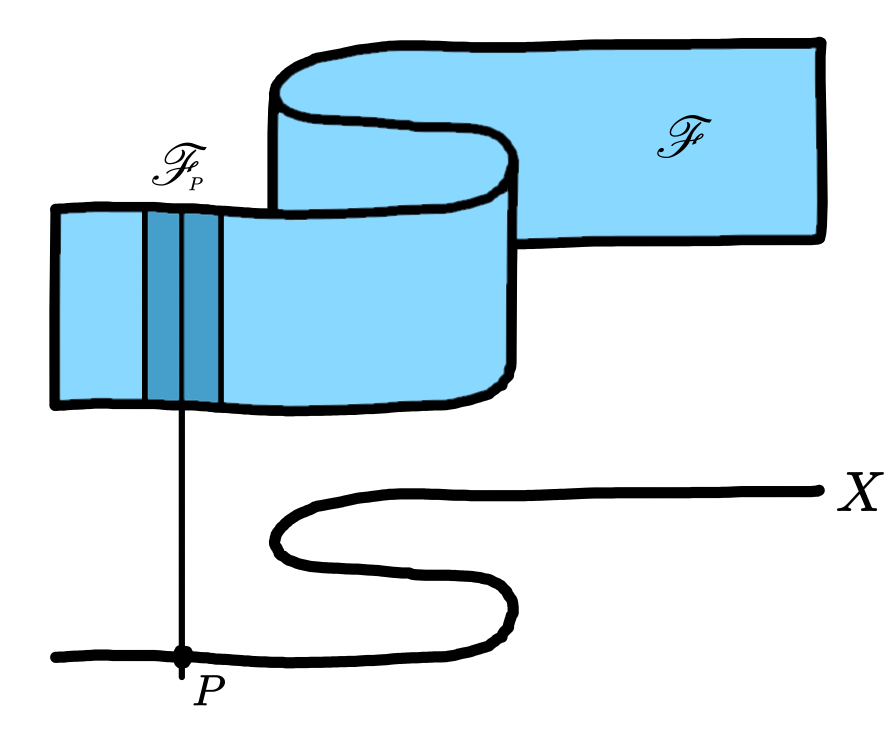
\includegraphics[width=\textwidth]{cover}
\end{figure}
\newpage
\tableofcontents

\theoremstyle{plain}
\newtheorem{thm}{Theorem}[section]
\newtheorem{cor}{Corollary}[thm]
\newtheorem{prop}[thm]{Proposition}
\newtheorem{lemm}[thm]{Lemma}
\newtheorem*{rem}{Remark}
\newtheorem*{claim}{Claim}
\theoremstyle{definition}
\newtheorem{defin}[thm]{Definition}
\newtheorem{ex}[thm]{Example}

\tcbset{beforeafter skip=8pt, toptitle=2pt, bottomtitle=2pt}
\newtcolorbox{cat}{colback=blue!2!white, colframe=blue!75!white, title=\emoji{warning} Abstract nonsense ahead}
\newtcolorbox{bcat}{colback=blue!2!white, colframe=blue!75!white, breakable, title=\emoji{warning} Abstract nonsense ahead}
\newtcolorbox{lnote}{colback=white, colframe=yellow!90!black, center}
\newtcbox{\note}{colback=white, colframe=yellow!90!black, center}
\newtcolorbox{lwarn}{colback=white, colframe=red!90!black, center}
\newtcbox{\warn}{colback=white, colframe=red!90!black, center}

\renewcommand{\phi}{\varphi}
\newcommand{\diffs}[1]{\Omega\left(#1\right)}
\newcommand{\dual}[1]{H^1(X,\mathcal{L}\left(#1\right))^{\vee}}
\newcommand{\duals}{H^1(X,\mathcal{L}(\kern.08em\bullet\kern.08em))^{\vee}}
\renewcommand{\emptyset}{\text{\O}}
\newcommand{\cm}{\widetilde{M}}

\section*{Introduction}
\addcontentsline{toc}{section}{Introduction}
In this article, I am introducing sheaf theory and the cohomology of
sheaves in the context of algebraic geometry to prove the Riemann-Roch 
theorem, which is one of the most important theorems in the classification
of algebraic curves. This text is aimed at undergraduate students with
basic knowledge of varieties.

Sheaves are formed by attaching algebraic data to \emph{local} patches of 
a space. We usually associate data about rational functions, and 
the Riemann-Roch theorem will give \emph{global} information about certain 
types of functions on a space. I will use the theorem to show the existence 
of a globally defined function on a curve $X$ of genus 0, which defines 
an isomorphism with the projective line. Thus, we get a complete 
classification of curves of genus 0. One can use the Riemann-Roch theorem 
to classify curves of higher genera as well.

The main ingredient in the proof of the Riemann-Roch theorem is Serre
Duality, which is a more general result. The proof will again
be cohomological and is usually rather abstract. However, I will
approach the proof by giving concrete interpretations of
the cohomology groups by following Serre's exposition in \cite{serre}.

The reader is assumed to know basic algebraic geometry. An excellent
introduction to the topic is \cite{reid}, and a good set of lecture notes
which goes beyond the basics is \cite{gathmann}. I will use the language
of discrete valuation rings, which is not explained in this paper. See
\cite{fulton} for an introduction to this topic. Having familiarity with 
the basic constructions of homological algebra is desirable. Throughout 
the paper, I will also try to point out category theoretical contexts of
the concepts discussed. However, it is not necessary to know any category
theory to understand this paper, and I will always place a warning for
people who are not fond of abstract nonsense.

\section{Sheaves}
The central objects of study in this paper are \emph{sheaves}. At first
glance sheaves might seem complicated and abstract, but in fact they are
inherently geometric objects. Hence, I will not start by stating the
definitions of sheaves, but instead I start with a discussion of
\emph{fibre bundles}, which are more concrete objects that appear through
out geometry. I hope this discussion gives a good motivation for
the definition of sheaves and also helps build geometric intuition right
away.

\subsection{Motivation: fibre bundles}
The idea of a fibre bundle is to attach some space, called a \emph{fibre}
$F$, to every point of some topological space $B$, which will be called
the \emph{base space} \cite{hatcher}. When we attach the fibres to the
points of $B$, we should get a topological space $E$ called the
\emph{total space}. More formally, a fibre bundle consists of two spaces $E$
and $B$ and a continuous surjection (henceforth \emph{a projection})
$\pi:E\to B$, where the fibres $\pi^{-1}(b)$ of the projection are
homeomorphic to some fibre space $F$. But not only that, we also require
that one can find an open neighbourhood $U$ for every point of $B$ and a
homeomorphism $h:\pi^{-1}(U)\to U\times F$ such that the following diagram
commutes.
\begin{figure}[H]
  \centering
  \begin{minipage}{.45\textwidth}
    \centering
    \begin{tikzcd}[row sep=large, column sep=small]
      {\pi^{-1}(U)} && {U\times F} \\
      & U
      \arrow["\pi"', from=1-1, to=2-2]
      \arrow["{\text{proj}_1}", from=1-3, to=2-2]
      \arrow["h", leftrightarrow, from=1-1, to=1-3]
    \end{tikzcd}
  \end{minipage}%
  \begin{minipage}{.45\textwidth}
    \centering
    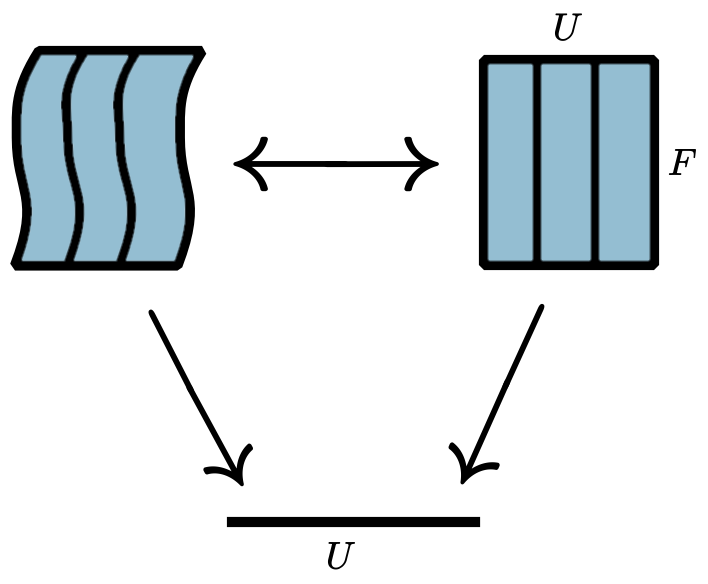
\includegraphics[width=.7\textwidth]{fibre_bundle}
  \end{minipage}
\end{figure}
Thus, when we attach the fibres to points of $B$, they should be gathered
so that the total space looks locally like a product space.

Let us look at some examples. Suppose the base space is the circle $S^{1}$
and the fibre space is the interval $[-1, 1]$, which is topologically
speaking a line. An example of such a \emph{line bundle} is the cylinder.
The cylinder is a \emph{trivial bundle}, because the whole space can
be written as a product: $S^{1}\times [-1,1]$. An example of a
\emph{non-trivial line bundle} over $S^{1}$ is the \emph{Möbius strip}.
\begin{figure}[H]
  \centering
  \begin{minipage}{.45\textwidth}
    \centering
    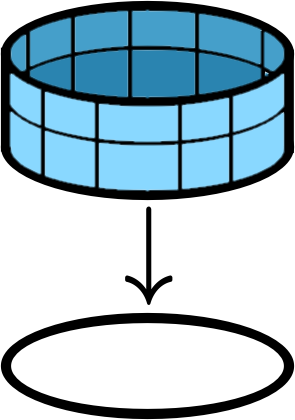
\includegraphics[height=4cm]{cylinder}
  \end{minipage}%
  \begin{minipage}{.45\textwidth}
    \centering
    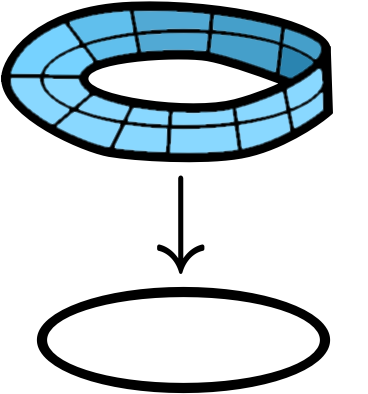
\includegraphics[height=4cm]{mobius}
  \end{minipage}
  \caption{The two line bundles over $S^{1}$}
\end{figure}
Similarly, we can consider \emph{circle bundles} over $S^{1}$. A trivial
circle bundle over $S^{1}$ is the torus and a non-trivial example is given
by the \emph{Klein bottle}.
An important example showing up in differential and algebraic geometry
is the concept of the \emph{tangent bundle}, where the fibres are the
tangent spaces at the points of the base space. Consider for example the
sphere $S^{2}$, which is a smooth 2-manifold. Then the fibres of the tangent
bundle of $S^{2}$ are the planes tangent to the sphere.

The things we are usually the most interested in are the \emph{sections} of
a given fibre bundle. A section $s$ of a fibre bundle $\pi:E\to B$
is a continuous map $s:B\to E$ such that $\forall b\in B,\ \pi(s(b))=b$.
This condition ensures that $s$ maps every point of the base space to the
corresponding fibre. A useful analogy is to think of a river, which can
be represented by a curve $C$ on the Euclidean plane. One could measure the
temperature of the river at different points and get a temperature reading
in $\mathbb{R}^{+}$ (assuming the
\begin{wrapfigure}{r}{0.3\textwidth}
  \centering
  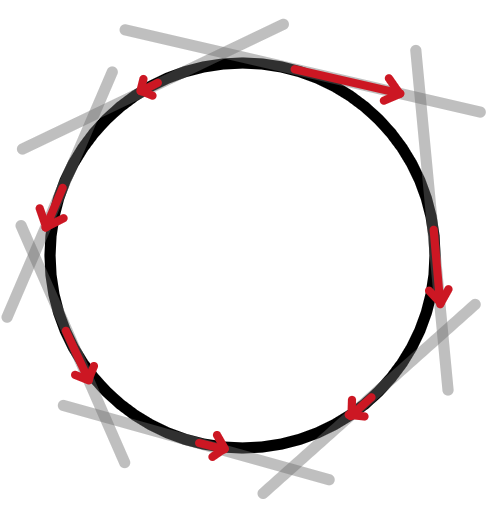
\includegraphics[width=0.3\textwidth]{vector_field}
  \caption{A section of the tangent bundle on $S^{1}$}
\end{wrapfigure}
 measurement is taken in Kelvins).
If one were to collect the temperature readings across all points of $C$,
one would get a section of the $\mathbb{R}^{+}$-bundle over the river $C$.
Thus, if fibre bundles are a way of attaching data to points of a space,
then sections of a fibre bundle are continuous collections of data over the
base space. One more interesting example is a section of a tangent bundle.
These are simply vector fields on the base space.
In practise, we also consider sections $s:U\to E$ on some open set
$U\subseteq B$, because given two sections $s_{1}:U_{1}\to E$ and
$s_{2}:U_{2}\to E$, we can glue the two sections proveded the sections
agree on $U_{1}\cap U_{2}$ to get a section $s:U_{1}\cup U_{2}\to E$.
Then, one can piece together larger sections from smaller sections. This
ability to define sections locally is very useful.

\subsection{Defining sheaves}
To summarise, fibre bundles are a way of attaching geometric data to
points of a given space, and one can consider sections over the fiber
bundle, which can be glued from small patches. We wish to extend the notion
of a fibre bundle, because the requirement that the fibres must be
topological spaces which form another topological space when bundled
together is more strict than we want. What if we want to consider, in
the above analogy, the types of fish living in the different parts of the
river? The set of types of fish does not form a topological space, but we
can still define a functions $s:U\to F$, where $F$ is the set of types
of fish and $U\subseteq C$ is an open set.

The notion of a fibre bundle is extended by the notion of a sheaf.
Since taking sections is really the interesting part of fibre bundles, the
definition of a sheaf will not be built with fibres and projection maps
but with sections. For the rest of this section, I use \cite{gathmann} as
my main source for sheaf theoretic results. Next I will state the formal
definition of a \emph{pre-sheaf}. Pay attention to the properties that are
motivated by fibre bundles.
\begin{defin}
  A pre-sheaf $\mathscr{F}$ of sets on a topological space $X$ associates
  to each open set $U\subseteq X$ a set $\mathscr{F}(U)$, which is called
  the set of sections over $U$. For every pair of nested open sets
  $V\subseteq U$, one defines a function
  $\text{res}_{V}^{U}:\mathscr{F}(U)\to\mathscr{F}(V)$,
  called the restriction function, such that $\text{res}_{U}^{U}
  =\text{id}_{U}$ and for every triple $W\subseteq V\subseteq U$, we have
  $\text{res}_{W}^{V}\circ\text{res}_{V}^{U}=\text{res}_{W}^{U}$.
  When $s\in\mathscr{F}(U)$, one usually writes $s\vert_{V}$ for
  $\res_{V}^{U}(s)$. Also, the set of global sections $\mathscr{F}(X)$
  is denoted by $\Gamma(\mathscr{F})$.

  One can also define pre-sheaves of rings, for example, where the sets
  $\mathscr{F}(U)$ are rings and the restriction functions are
  ring homomorphisms.
\end{defin}
Note that pre-sheaves generalise the concept of taking sections on a
topological space, but this definition doesn't capture the important property
that sections should be able to be glued if they agree on the intersection.
Thus, sheaves are defined in the following way.
\begin{defin}
  A pre-sheaf $\mathscr{F}$ is a sheaf if the following property holds.
  Suppose $U\subseteq X$ is an open set with an open cover $(U_{i})_{i\in I}$.
  If $s_{i}\in\mathscr{F}(U_{i})$ are sections such that
  $s_{i}\vert_{U_{i}\cap U_{j}}=s_{j}\vert_{U_{i}\cap U_{j}}$ for all pairs $i$
  and $j$, then there is a unique section $s\in\mathscr{F}(U)$ such that
  $\forall i\in I,\ s\vert_{U_{i}}=s_{i}$.
\end{defin}
\begin{bcat}
  Category theoretically speaking, a pre-sheaf $\mathscr{F}$ of sets is
  simply a contravariant functor $\mathscr{F}:\text{Op}(X)^{\text{op}}
  \to\mathbf{Set}$, where $\text{Op}(X)$ is the posetal category of
  open sets of $X$. Moreover, a pre-sheaf of rings is a contravariant functor
  $\mathscr{F}:\text{Op}(X)^{\text{op}}\to \mathbf{Ring}$, and in general,
  a $\mathscr{C}$-valued pre-sheaf is a contravariant functor
  $\mathscr{F}:\text{Op}(X)^{\text{op}}\to\mathscr{C}$, where we define
  $\mathscr{F}(\emptyset)$ to be the final object of $\mathscr{C}$.
  If $\mathscr{C}$ has limits, we can also express the sheaf axiom category
  theoretically. Namely, $\mathscr{F}$ is a sheaf if for every
  open set $U$ of $X$ and an open cover $U_{i}$ of $U$ the following
  diagram is an equaliser diagram.
  \begin{equation}\label{diag:sheaf_eq}\begin{tikzcd}
      \mathscr{F}(U)\rar
      & \displaystyle\prod_{i}\mathscr{F}(U_{i})\rar[shift left]\rar[shift right]
      & \displaystyle\prod_{i,j}\mathscr{F}(U_{i}\cap U_{j})
    \end{tikzcd},\end{equation}
  where the first map is the product of the restrictions
  $\text{res}_{U_{i}}^{U}$ and the pair of maps are products of the
  restrictions $\text{res}_{U_{i}\cap U_{j}}^{U_{i}}$ and
  $\text{res}_{U_{i}\cap U_{j}}^{U_{j}}$ respectively.
\end{bcat}

Next, suppose $\pi: E\to B$ is a fibre bundle. One can easily check that
it is possible to define a sheaf $\mathscr{F}$ by
\[
  \mathscr{F}(U) = \Set{s:U\to E\mid s\text{ a section of }\pi}.
\]
An example of a sheaf showing up in algebraic geometry is the structure
sheaf $\mathscr{O}_{X}$ of an affine variety $X$ defined by
\[
  \mathscr{O}_{X}(U)=\Set{f\in k(X)\mid f\text{ regular on } U}.
\]
From now on, we will be concentrating on this sheaf more.

\subsection{Stalks and sheafification}
Now I will introduce two important constructions: stalks, which give a
zoomed-in picture of a sheaf, and sheafification, which turns pre-sheaves
into sheaves.

\begin{defin}
  Given a pre-sheaf $\mathscr{F}$ on $X$ and a point $P\in X$, the stalk
  $\mathscr{F}_{P}$ at $P$ is defined as the set
  \[
    \mathscr{F}_{P}=\Set{(s, U)\mid U\subseteq X\text{ open}, s\in
    \mathscr{F}(U)}/\sim,
  \]
  where two pairs $(s_{1}, U_{1})$ and $(s_{2}, U_{2})$ are equivalent
  if there is an open set $V\subseteq U_{1}, U_{2}$ such that
  \[
    s_{1}\vert_{V}=s_{2}\vert_{V}.
  \]
  The equivalence class of a pair $(s, U)$ is called the \emph{germ}
  of $s$ at $P$. Given a section $s\in\mathscr{F}(U)$, its germ at $P$
  is usually denoted by $s_{P}$.
\end{defin}
\begin{cat}
  The stalks can be written as the direct limit
  \[\mathscr{F}_{P}=\varinjlim_{U\ni P}\mathscr{F}(U).\]
\end{cat}
Next I will do an example computation with stalks, which will be useful
later.
\begin{prop}
  Let $X$ be an affine variety. The stalk $\mathscr{O}_{X,P}$ of
  $\mathscr{O}_{X}$ at some point $P\in X$ is given by
  \[
    \mathscr{O}_{X,P}=\Set{\frac{f}g\in k(X)\mid g(P)\neq 0}.
  \]
\end{prop}
\begin{proof}
  I will prove the two inclusions separately.
  \begin{description}[style=nextline]
    \item[$\subseteq\big)$]
          Let $[(\phi, U)]\in \mathscr{O}_{X,P}$. Since $P\in U$ and
          $\phi\in \mathscr{O}(U)$, $\phi$ must be regular at $P$. Thus,
          $\phi$ has a representation $\frac{f}g$ as a rational function
          around $P$, where $g(P)\neq 0$. Moreover, if $[(\phi_{1}, U_{1})]
          =[(\phi_{2}, U_{2})]$, then there is an open set $V\subseteq
          U_{1},U_{2}$ such that $\phi_{1}\vert_{V}=\phi_{2}\vert_{V}$.
          Therefore, $\phi_{1}$ and $\phi_{2}$ can be represented by the
          same rational function around $P$.
    \item[$\supseteq\big)$]
          Now suppose $\frac{f}g\in k(X)$ with $g(P)\neq 0$. Then, there
          is an open neighbourhood $U$ of $P$ where $g$ is non-zero.
          Clearly, $(\frac{f}g, U)$ defines a germ in $\mathscr{O}_{X,P}$.
  \end{description}
\end{proof}

The stalks of a sheaf are analogous to the fibres of a fibre bundle.
Just as a section of a fibre bundle takes values in the fibres, a section of
a sheaf takes values in the stalks.
\begin{figure}[H]
  \centering
  \begin{minipage}{.5\textwidth}
    \centering
    \begin{lwarn}
      Note however that while a stalk at $P$ contains all the data ``above''
      $P$ just as a fibre at $P$ does, stalks are larger, because they also
      contain ``infinitesimal'' data \textbf{around} $P$. One can find two
      sections with equal values at $P$, but which have different germs at
      $P$.
    \end{lwarn}
  \end{minipage}%
  \begin{minipage}{.45\textwidth}
    \centering
    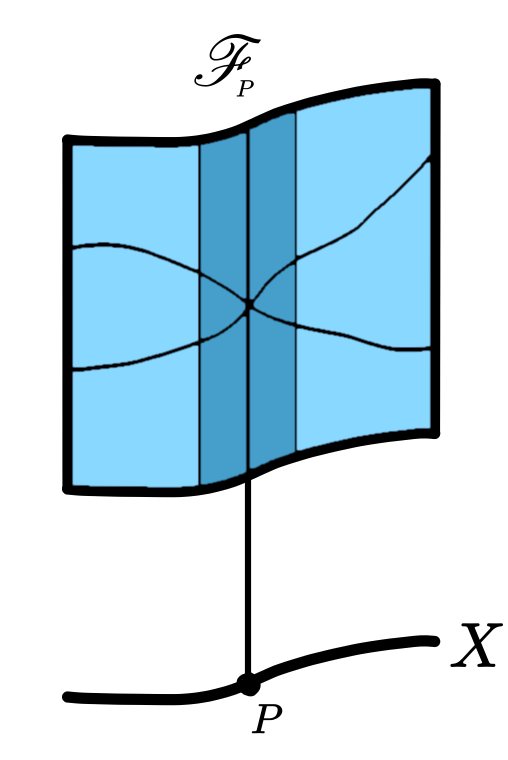
\includegraphics[width=.45\textwidth]{germs}
  \end{minipage}
\end{figure}
Fix a sheaf $\mathscr{F}$ on some space $X$ and choose a section
$s\in \mathscr{F}(U)$ on some open set $U\subseteq X$. Then, consider
the totality of germs of $s$ over $U$, namely the collection
$(s_{P})_{P\in U}$ with $s_{P}\in\mathscr{F}_{P}$. Since $\mathscr{F}$ is a
sheaf, it turns out that one can recover the section $s$ from the
germs: Each germ $s_{P}$ has a representative $(s\vert_{U_{P}}, U_{P})$.
The set $U$ is covered by the $U_{P}$ and since the $s\vert_{U_{P}}$ are
restrictions of the common section $s$ onto the sets $U_{P}$, one can use the
sheaf axiom to glue the sections $s\vert_{U_{P}}$ together and obtain a
section on $U$ which must be equal to $s$ by uniqueness. Generalising this
observation, one can write the sections of a sheaf as a collection of germs:
\begin{lemm}\label{lemm:sheafify_sheaf}
  Given a sheaf $\mathscr{F}$ on a space $X$, one can write
  \begin{align*}
    \mathscr{F}(U)=\big\{\,
    & (s_{P})_{P\in U}\,\big\vert\, s_{P}\in\mathscr{F}_{P}\text{ such that} \\
    & \forall P\in U\,
      \exists U_{P}\subseteq U\text{ an open neighbourhood of }P \\
    & \exists r\in\mathscr{F}(U_{P})\,\forall Q\in U_{P},\ r_{Q}=s_{Q}\,\big\}
  \end{align*}
  for every open set $U\subseteq X$
\end{lemm}
This statement may seem bewildering at first, but note that the important
part in the above observation was that when we fixed a point $P$, there was
an open set $U_{P}$ where all the germs $s_{Q}$ for $Q\in U_{P}$ agreed
with some section $s\vert_{U_{P}}$ on $U_{P}$. We want to ensure that this is
the case with the collection $(s_{P})_{P\in X}$ of the proposition so that we
can glue the germs in the same way as above. This statement will be essential
for building theory, but it is also useful for manipulating sheaves in
practise and I will routinely represent sections of sheaves as collections
of germs. Thus, make sure you understand the statement and the proof
completely.
\begin{proof}
  I will again break up the proof into cases.

  \begin{description}[style=nextline]
    \item[$\subseteq\big)$]
          Suppose $s\in\mathscr{F}(U)$ is a section on $U$. Fix an arbitrary
          point $P\in U$ and choose a representative $(s\vert_{U_{P}}, U_{P})$
          of the germ $s_{P}$ of $s$. If one takes $r=s\vert_{U_{P}}\in
          \mathscr{F}(U_{P})$, then it follows immediately that
          \[\forall Q\in U_{P},\ r_{Q}=s_{Q}.\]
    \item[$\supseteq\big)$]
          Now, suppose $(s_{P})_{P\in U}$ is a collection of germs in the
          RHS set. Then, $U$ is covered by the sets $U_{P}$ associated to
          each germ $s_{P}$. Now, fix two points $P_{1},P_{2}\in U$,
          and consider the associated sections $r_{1}\in\mathscr{F}(U_{P_{1}})$
          and $r_{2}\in\mathscr{F}(U_{P_{2}})$. It is clearly the case that
          $r_{1}\vert_{U_{P1}\cap U_{P2}}=r_{2}\vert_{U_{P1}\cap U_{P2}}$, because
          of the germs of $r_{1}$ and $r_{2}$ are related through the germs
          $s_{P}$ on $U_{P_{1}}\cap U_{P_{2}}$. Therefore, we can take all
          the sections $r_{P}\in\mathscr{F}(U_{P})$ associated to the germs
          $s_{P}$ and glue them together to obtain a section $s$ on $U$.
          The germs of this section are clearly the germs $s_{P}$.
  \end{description}
\end{proof}

Now, since one can take stalks of pre-sheaves too, one might try this
construction on a pre-sheaf. If $\mathscr{F}^{\prime}$ is a pre-sheaf
on some space $X$, one can define another pre-sheaf $\mathscr{F}$
on $X$ by
\begin{align*}
  \mathscr{F}(U)=\big\{\,
  & (s_{P})_{P\in U}\,\big\vert\, s_{P}\in\mathscr{F}_{P}^{\prime}
    \text{ such that} \\
  & \forall P\in U\,
    \exists U_{P}\subseteq U\text{ an open neighbourhood of }P \\
  & \exists r\in\mathscr{F}^{\prime}(U_{P})\,\forall Q\in U_{P},
    \ r_{Q}=s_{Q}\,\big\}.
\end{align*}
One may notice that $\mathscr{F}$ is in fact a sheaf. Thus, one can
associate a sheaf to every pre-sheaf using this construction, which is
called \emph{sheafification}. And Lemma~\ref{lemm:sheafify_sheaf} is saying
that sheafifying a sheaf does not do anything. One can also see that the
pre-sheaf $\mathscr{F}^{\prime}$ and its sheafification $\mathscr{F}$ always
have the same stalks.
\begin{rem}
  One might also notice that this construction preserves the stalks of
  $\mathscr{F}^{\prime}$. In other words, $\mathscr{F}^{\prime}_{P}
  =\mathscr{F}_{P}$ for every $P\in X$. This is true, because every
  element $(s, U)$ of $\mathscr{F}^{\prime}_{P}$ can be associated to
  the element $(s_{Q})_{Q\in U}$ of $\mathscr{F}(U)$, which in turn has
  a stalk at $P$ in $\mathscr{F}_{P}$ and an element $((s_{Q})_{Q\in U},
  U)$ of $\mathscr{F}_{P}$ can be associated to $s_{P}\in
  \mathscr{F}^{\prime}_{P}$.
\end{rem}
\begin{cat}
  If $\mathscr{F}^{\prime}$ is a pre-sheaf on $X$, then its sheafification
  $\mathscr{F}$ satisfies the following universal property: for every sheaf
  $\mathscr{G}$ and mophism $g:\mathscr{F}^{\prime}\to\mathscr{G}$, there
  exists a unique morphism $f:\mathscr{F}\to\mathscr{G}$ making the following
  diagram commute.
  \[\begin{tikzcd}
      \mathscr{F}^{\prime}\rar\arrow[dr, "g"'] & \mathscr{F}
      \arrow[d, dashed, "f"] \\ & \mathscr{G}
    \end{tikzcd}\]
  (Morphisms of sheaves will be defined in subsection~\ref{ss:sheaf_alg})

  Also, the sheafification functor $\mathbf{PSh}(X)\to\mathbf{Sh}(X)$
  from the category of pre-sheaves on $X$ to the category of sheaves on $X$
  is the left adjoint to the forgetful functor $\mathbf{Sh}(X)\to
  \mathbf{PSh}(X)$. % TODO: Cite nlab
\end{cat}
A typical example illustrating sheafification is to consider the constant
pre-sheaf and its sheafification. The constant pre-sheaf % TODO: Citation?
$\mathscr{F}^{\prime}$ on a space $X$ is defined as follows
\[
  \mathscr{F}^{\prime}(U) =\Set{c: U\to\mathbb{R}\mid c
    \text{ a constant function }}.
\]
One can see that this is not a sheaf: take any two disjoint open sets
$U_{1}, U_{2}\subseteq X$ and two constant functions $c_{1}:U_{1}\to
\mathbb{R}$ and $c_{2}:U_{2}\to\mathbb{R}$ with different values.
Then, the two sections don't glue to form a constant function on
$U_{1}\cup U_{2}$ (all of this assumes that $X$ is a space with
at least one pair of disjoint open sets). The sheafification $\mathscr{F}$ of
$\mathscr{F}^{\prime}$ is given by sections $(c_{P})_{P\in U}$. By the
definition of sheafification, there is for every $P\in U$ an open
neighbourhood $U_{P}\subseteq U$ of $P$ and a constant function
$d: U_{P}\to\mathbb{R}$ such that $\forall Q\in U_{P},\ c_{Q}=d_{Q}$.
Hence, the restriction of $(c_{Q})_{Q\in U}$ to $U_{P}$ can be identified
with the constant function $d$. Therefore, the sheafification of the constant
pre-sheaf constists of \emph{locally constant functions}. In general, given
a set $A$, the constant sheaf $\underline{A}$ is defined as the sheafification
of the constant pre-sheaf with values in $A$.

Now is a good time to introduce other sheaves that will be needed later.
First one is the \emph{skyscraper sheaf} of some set $A$ at a point $P\in X$.
It is defined as follows
\[
  A_{P}(U)=\begin{cases}
    A, & \quad P\in U \\
    0, & \quad P\not\in U
  \end{cases}.
\]
A second sheaf we need is the \emph{restriction sheaf} of some other sheaf.
Suppose $\mathscr{F}$ is a sheaf on some space $X$ and $U\subseteq X$ is
an open set. Then, one defines the restriction sheaf $\mathscr{F}\vert_{U}$
on $U$ simply by
\[
  \mathscr{F}\vert_{U}(V)=\mathscr{F}(V)
\]
for open sets $V\subseteq U$.

\subsection{Ringed spaces and algebraic varieties}
Now that we have some feel for sheaves, I will briefly go over the
construction of abstract algebraic varieties, which are built with the help
of sheaves. Whenever I mention varieties, I refer to the spaces that are
defined in this subsection. The precise details of the construction are not
essential for the present article, and the reader should consult
\cite{gathmann} for a more detailed discussion.

In geometry, one is not only interested in the points of the space,
but also in the functions on the space. Thus, I will extend the notion of
a topological space by attaching the data of the functions on the space.
\begin{defin}
  A ringed space is a pair $(X,\mathscr{O}_{X})$ consisting of a topological
  space $X$ and a sheaf of rings $\mathscr{O}_{X}$ called the structure
  sheaf of $X$.
\end{defin}
Next, I will define morphisms between ringed spaces following the
definition given in \cite{gathmann}.
\begin{defin}
  Suppose $(X,\mathscr{O}_{X})$ and $(Y,\mathscr{O}_{Y})$ are two ringed
  spaces with structure sheaves consisting of $k$-valued functions
  for some field $k$. Then a morphism from $(X,\mathscr{O}_{X})$ to
  $(Y,\mathscr{O}_{Y})$ is a (set-theoretic) continuous map
  $f:X\to Y$ such that
  \begin{equation}\label{eq:ring_spc_morph}
    \forall U\subseteq Y\text{ open},\ f^{\ast}\mathscr{O}_{Y}(U)
    \subseteq \mathscr{O}_{X}(f^{-1}(U)),
  \end{equation}
  where $f^{\ast}g=g\circ f$ for $g\in\mathscr{O}_{Y}(U)$.
\end{defin}
To understand the condition in \eqref{eq:ring_spc_morph}, it helps to look
at the following commutative diagram.
\[\begin{tikzcd}[column sep=small]
    {X} && {Y} \\
    & k
    \arrow["{f^{\ast}g}"', from=1-1, to=2-2]
    \arrow["g", from=1-3, to=2-2]
    \arrow["f", from=1-1, to=1-3]
  \end{tikzcd}\]
The condition requires that functions $g\in\mathscr{O}_{Y}(U)$ ``pull back''
to functions in $\mathscr{O}_{X}(f^{-1}(U))$ along the map $f:X\to Y$. As
usual, one can define isomorphisms of ringed spaces as morphisms
$f:(X,\mathscr{O}_{X})\to (Y,\mathscr{O}_{Y})$ such that there is a morphism
$g:(Y,\mathscr{O}_{Y})\to (X,\mathscr{O}_{X})$ with $f\circ g=g\circ f
=\text{id}$. Next I will define what it means for a ringed space to be
an affine variety.

\begin{defin}[Def. 2.3.15 in \cite{gathmann}]
  A ringed space $(X,\mathscr{O}_{X})$ is an affine variety if
  \begin{itemize}
    \item $X$ is an irreducible space,
    \item $\mathscr{O}_{X}$ is a sheaf of $k$-valued functions,
    \item There is an irreducible algebraic set $Y\subseteq \mathbb{A}^{n}$
          such that $(X,\mathscr{O}_{X})\cong (Y,\mathscr{O}_{Y})$.
  \end{itemize}
\end{defin}
Note that such ringed spaces are not always zero sets of some polynomials;
See for example Lemma 2.3.16 in \cite{gathmann}.

Now that I have defined what it means for a ringed space to be an affine
variety, I will form \emph{varieties} by ``gluing'' up open affine varieties
in the same way as manifolds are glued from open subsets of the Euclidean
space.
\begin{defin}[Def. 2.4.1 in \cite{gathmann}]
  A ringed space $(X,\mathscr{O}_{X})$ is a pre-variety if
  \begin{itemize}
    \item $X$ is an irreducible space,
    \item $\mathscr{O}_{X}$ is a sheaf of $k$-valued functions,
    \item $X$ can be covered with finitely many open sets $U_{i}$
          such that each $(U_{i},\mathscr{O}_{X}\vert_{U_{i}})$ is
          an affine variety.
  \end{itemize}
\end{defin}
The reason why these spaces are not yet varieties, but only pre-varieties
is because the definition allows the construction of some pathological
spaces such as the \emph{line with two origins}, see \cite{gathmann}.
To avoid such spaces, we add one more condition in the final definition
of a variety.
\begin{defin}[Def. 2.5.1 in \cite{gathmann}]
  A pre-variety $X$ is a variety, if for every pre-variety $Y$ and any
  pair of morphisms $f_{1}, f_{2}: Y\to X$, the set
  $\set{P\in Y\mid f_{1}(P)=f_{2}(P)}$ is closed in $Y$.
\end{defin}
Let me prove a small lemma about affine subsets of a variety.
\begin{lemm}\label{lemm:affine_intersection}
  Suppose $X$ is a variety and $U, V\subseteq X$ are two affine subsets.
  Then, the intersection $U\cap V$ is affine.
\end{lemm}
\begin{proof}
  TODO.
\end{proof}

\subsection{Algebraic constructions with sheaves}\label{ss:sheaf_alg}
The aim of this subsection is to define algebraic constructions for
sheaves so that we can study them using the tools of
\emph{homological algebra}. First I need to define morphisms between
pre-sheaves.
\begin{defin}
  Suppose $\mathscr{F}$ and $\mathscr{G}$ are pre-sheaves of sets or rings
  on some space $X$. Then, a morphism $\alpha:\mathscr{F}\to\mathscr{G}$
  consists of set functions or ring homomorphisms
  $\alpha_{U}:\mathscr{F}(U)\to\mathscr{G}(U)$ which commute with restriction
  maps. That is, the following diagrams commute.
  \[\begin{tikzcd}
      \mathscr{F}(U)\rar{\text{res}_{V}^{U}}\arrow[d, "\alpha_{U}"']
      & \mathscr{F}(V)\dar{\alpha_{V}} \\
      \mathscr{G}(U)\arrow[r,"\text{res}_{V}^{U}"'] & \mathscr{G}(V)
    \end{tikzcd}\]
  If $\mathscr{F}$ and $\mathscr{G}$ are sheaves, a sheaf morphism is defined
  exactly the same way.
\end{defin}
One might ask, why this should be the right definition. The reason is that
this type of morphism \textbf{preserves the structure of the sheaf}. Compare
this with group homomorphisms. Firstly, a group homomorhism $\phi:G\to H$
associates to every element of $G$ a corresponding element in $H$. In the
same way a sheaf morphism $\alpha$ must associate to every section
$s\in\mathscr{F}(U)$ a corresponding section $\alpha_{U}(s)\in\mathscr{G}(U)$
of $\mathscr{G}$. Secondly, if three elements of the group are related by
the group structure so that $a\cdot b = c$, then the homomorphism should
respect this structure so that $\phi(a)\cdot\phi(b)=\phi(c)$. Similarly,
the sheaf morphism $\alpha$ should respect the structure of the sheaves
given by the restriction maps: if $s\vert_{V}=r$, then $\alpha(s)\vert_{V}
=\alpha(r)$.
\begin{cat}
  As one can immediately see, morphisms of pre-sheaves and sheaves are simply
  natural transformations of contravariant functors.
\end{cat}

In order to proceed to define algebraic constructions on sheaves, I must
restrict to some class of sheaves with an algebraic structure. The class
usually considered in algebraic geometry is the class of
\emph{sheaves of $\mathscr{O}_{X}$-modules} on a ringed space
$(X,\mathscr{O}_{X})$.
\begin{defin}
  Given a ringed space $(X,\mathscr{O}_{X})$, a sheaf $\mathscr{F}$ on $X$
  is a sheaf of $\mathscr{O}_{X}$-modules, if the sets $\mathscr{F}(U)$
  are $\mathscr{O}_{X}(U)$-modules and the restriction maps satisfy the
  following condition. Suppose $V\subseteq U\subseteq X$ are open and
  $s,s_{1}, s_{2}\in\mathscr{F}(U)$ are sections. Then,
  \[
    (s_{1}+s_{2})\vert_{V}=s_{1}\vert_{V}+s_{2}\vert_{V}\quad
    \text{and}\quad (\lambda s)\vert_{V}=\lambda\vert_{V}\cdot s\vert_{V}
  \]
  for all scalars $\lambda\in\mathscr{O}_{X}$.
\end{defin}
I can now define the usual algebraic operations for sheaves of
$\mathscr{O}_{X}$-modules.
\begin{defin}\label{def:sheaf_algebra}
  Suppose $\mathscr{F}_{1}$ and $\mathscr{F}_{2}$ are sheaves of
  $\mathscr{O}_{X}$-modules and $f:\mathscr{F}_{1}\to\mathscr{F}_{2}$ is a
  morphism of sheaves. Then the sheaves $\ker f$, $\coker f$,$\im f$,
  $\mathscr{F}_{1}\oplus\mathscr{F}_{2}$, $\mathscr{F}_{1}\otimes
  \mathscr{F}_{2}$, and $\mathscr{F}_{1}^{\vee}$ are defined as the
  sheafifications of the corresponding pre-sheaves given by the following:
  \begin{enumerate}
    \item $(\ker^{\prime} f)(U) = \ker(f_{U}:\mathscr{F}_{1}(U)
          \to\mathscr{F}_{2}(U))$
    \item $(\coker^{\prime} f)(U) = \coker(f_{U}:\mathscr{F}_{1}(U)
          \to\mathscr{F}_{2}(U))$
    \item $(\im^{\prime} f)(U)=\im(f_{U}:\mathscr{F}_{1}(U)
          \to\mathscr{F}_{2}(U))$
    \item $(\mathscr{F}_{1}\oplus^{\prime}\mathscr{F}_{2})(U)=\mathscr{F}_{1}(U)
          \oplus\mathscr{F}_{2}(U)$
    \item $(\mathscr{F}_{1}\otimes^{\prime}\mathscr{F}_{2})(U)
          =\mathscr{F}_{1}(U)\otimes_{\mathscr{O}_{X}(U)}\mathscr{F}_{2}(U)$
    \item $\mathscr{F}_{1}^{\vee\prime}(U)=\text{Hom}_{\mathscr{O}_{X}(U)}(
          \mathscr{F}_{1}(U),\mathscr{O}_{X}(U))$
  \end{enumerate}
\end{defin}
One can actually check that the pre-sheaves $\ker^{\prime} f$ and
$\mathscr{F}_{1}\oplus^{\prime}\mathscr{F}_{2}$ are in fact already sheaves,
so sheafification doesn't change the definition. We also have the following
usual definitions.
\begin{defin}\hfill

  \begin{enumerate}
    \item A morphism $f:\mathscr{F}_{1}\to\mathscr{F}_{2}$ of sheaves of
          $\mathscr{O}_{X}$-modules is injective if $\ker f = 0$ and
          surjective if $\coker f = 0$.
    \item If $f$ is injective, we write $\mathscr{F}_{2}/\mathscr{F}_{1}$
          for the cokernel.
    \item A sequence
          \[\begin{tikzcd}
              \cdots\rar & \mathscr{F}_{i-1}\rar & \mathscr{F}_{i}\rar
              & \mathscr{F}_{i+1}\rar & \cdots
            \end{tikzcd}\]
          of $\mathscr{O}_{X}$-modules is exact if
          \[
          \ker(\mathscr{F}_{i}\to\mathscr{F}_{i+1})=\im(\mathscr{F}_{i-1}
          \to\mathscr{F}_{i}),\ \forall i.
          \]
  \end{enumerate}

\end{defin}
\begin{cat}
  One can show that the category $\mathscr{O}_{X}$\textbf{-Mod} of sheaves
  of $\mathscr{O}_{X}$-modules is an \emph{abelian category}, which means
  that it is the perfect setting for homological algebra (see \cite{vakil}).

  % TODO: Reference for the below result
  Furthermore, note that equaliser diagrams in abelian categories can be
  expressed in terms of exact sequences. Therefore, the sheaf axiom in
  \eqref{diag:sheaf_eq} can be expressed as the exact sequence
  \begin{equation}\label{diag:sheaf_ex}\begin{tikzcd}
      0\rar & \mathscr{F}(U)\rar & \displaystyle\prod_{i}\mathscr{F}(U_{i})
      \rar{\text{res}_{U_{i}\cap U_{j}}^{U_{j}}-\text{res}_{U_{i}\cap U_{j}}^{ U_{i}}}
      &[5em] \displaystyle\prod_{i,j}\mathscr{F}(U_{i}\cap U_{j})
    \end{tikzcd}\end{equation}
  in the category $\mathscr{O}_{X}$\textbf{-Mod}.
\end{cat}

Next I will show that the exactness of sequences of sheaves
is a local property. To see this, one should first note that a morphism
$f:\mathscr{F}_{1}\to\mathscr{F}_{2}$ of sheaves of
$\mathscr{O}_{X}$-modules induces an $\mathscr{O}_{X,P}$-module homomorphism
\[
  f_{P}:\left(\mathscr{F}_{1}\right)_{P}\to\left(\mathscr{F}_{2}\right)_{P}
  :[(s,U)]\mapsto [(f_{U}(s),U)]
\]
on the stalks. Then one can show the following theorem.
\begin{thm}[Lemma 13.21 in \cite{gathmann_new}]\label{thm:ses_equivalence}
  A sequence
  \[\begin{tikzcd}
      \cdots\rar{f_{i-2}} & \mathscr{F}_{i-1}\rar{f_{i-1}}
      & \mathscr{F}_{i}\rar{f_{i}} & \mathscr{F}_{i+1}\rar{f_{i+1}} & \cdots
    \end{tikzcd}\]
  of sheaves of $\mathscr{O}_{X}$-modules is exact if and only if the
  induced sequences
  \[\begin{tikzcd}
      \cdots\rar{\left(f_{i-2}\right)_{P}}
      & (\mathscr{F}_{i-1})_{P}\rar{\left(f_{i-1}\right)_{P}}
      & (\mathscr{F}_{i})_{P}\rar{\left(f_{i}\right)_{P}}
      & (\mathscr{F}_{i+1})_{P}\rar{\left(f_{i+1}\right)_{P}} & \cdots
    \end{tikzcd}\]
  on the stalks are all exact.
\end{thm}
\begin{proof}
  I will prove the two directions of the equivalence separately.
  \begin{description}[style=nextline]
    \item[$\Longrightarrow\big)$]
          The exactness of the first sequence implies
          that $\ker(f_{i})=\im(f_{i-1})$. Thus $\left(\ker(f_{i})\right)_{P}
          =\left(\im(f_{i-1})\right)_{P}$, and so
          \begin{align*}
            [(s, U)]\in\ker\left(\left(f_{i}\right)_{P}\right)
            &\iff \exists V\subseteq U,\ s\vert_{V}\in\ker^{\prime}(f_{i})(V)\\
            &\iff [(s\vert_{V},V)]\in\left(\ker(f_{i})\right)_{P} \\
            &\iff [(s\vert_{V},V)]\in\left(\im(f_{i-1})\right)_{P} \\
            &\iff \exists V\subseteq U,\ s\vert_{V}\in
              \im^{\prime}(f_{i-1})(V) \\
            &\iff [(s,U)]\in\im\left(\left(f_{i-1}\right)_{P}\right),
          \end{align*}
          where the second and fourth equivalences are left as exercises.
          Therefore, $\ker\left(\left(f_{i}\right)_{P}\right)
          =\im\left(\left(f_{i-1}\right)_{P}\right)$
          % TODO: Picture with exact sequence ker(f_i) -> F_i -> F_i+1
          %       and corresponding stalks
    \item[$\Longleftarrow\big)$]
          Choose an arbitrary open set $U\subseteq X$. Then,
          \begin{align*}
            s\in\ker(f_{i})(U)
            &\iff \forall P\in U,\ s_{P}\in\ker\left(\left(
              f_{i}\right)_{P}\right) \\
            &\iff \forall P\in U,\ s_{P}\in\im\left(\left(
              f_{i-1}\right)_{P}\right) \\
            &\iff s\in\im(f_{i-1})(U).
          \end{align*}
          In the first and the last equivalence one uses
          Lemma~\ref{lemm:sheafify_sheaf} to break the section $s$ into
          its germs and piece them back together. Thus,
          $\ker(f_{i})(U)=\im(f_{i-1})(U)$ for all open sets
          $U\subseteq X$, which implies that the sheaves are equal.
  \end{description}
\end{proof} % TODO: Add a picture to clarify this proof
One can prove the following results as an immediate corollary.
\begin{cor}
  Suppose $f:\mathscr{F}\to\mathscr{G}$ is a morphism of sheaves of
  $\mathscr{O}_{X}$-modules, and let $f_{P}:\mathscr{F}_{P}\to\mathscr{G}_{P}$
  be the induced homomorphism. Then,
  \begin{enumerate}
    \item $f$ is an injection iff $f_{P}$ is an injection,
    \item $f$ is a surjection iff $f_{P}$ is a surjection,
    \item $f$ is an isomorphism iff $f_{P}$ is an isomorphism.
  \end{enumerate}
\end{cor}

In algebraic geometry, one further restricts attention to a certain class of
sheaves of $\mathscr{O}_{X}$-modules called \emph{quasi-coherent sheaves}.
These have even nicer algebraic properties, and they include most sheaves
one encounters in algebraic geometry. To define quasi-coherent sheaves,
I need to first make the following definition, which generalises the
definition of the structure sheaf on an affine variety.
\begin{defin}
  Suppose $X$ is an affine variety and $M$ is a module over the coordinate
  ring $\mathscr{O}_{X}(X)$. Then, the sheaf $\cm$ associated with the
  module $M$ is defined as follows.
  \begin{align*}
    \cm(U)=\big\{\,
    & (\phi_{P})_{P\in U}\,\big\vert\, \phi_{P}\in M_{\mathfrak{m}_{P}}
      \text{ such that} \\
    & \forall P\in U\,
      \exists U_{P}\subseteq U\text{ an open neighbourhood of }P \\
    & \exists m\in M\,\exists g\in k[X]\,
    \forall Q\in U_{P},\ \phi_{Q}=\frac{m}g\text{ and } g(Q)\neq 0\,\big\},
  \end{align*}
  where $M_{\mathfrak{m}_{P}}$ is the localisation of $M$ at the maximal ideal
  $\mathfrak{m}_{P}$ of the point $P$.
\end{defin}
Now, this definition implies the following result.
\begin{lemm}\label{lemm:qcoh_local_global}
  If $\cm$ is the sheaf on an affine variety $X$ associated to the module
  $M$ over $\mathscr{O}_{X}(X)$, then
  \begin{enumerate}[label=\normalfont(\alph*)]
    \item $\forall P\in X, \left(\cm\right)_{P}=M_{\mathfrak{m}_{P}}$, and
    \item $\Gamma\left(\cm\right)=M$.
  \end{enumerate}
\end{lemm}
\begin{proof}
  TODO.
\end{proof}
Quasi-coherent sheaves are then constructed from such sheaves.
\begin{defin}
  A sheaf $\mathscr{F}$ of $\mathscr{O}_{X}$-modules is quasi-coherent, if
  for everey affine open set $U\subseteq X$, the sheaf $\mathscr{F}\vert_{U}$
  is a sheaf associated to some module $M$ over the coordinate ring
  $\mathscr{O}_{X}(U)$.
\end{defin}
\begin{rem} % TODO: Be more precise
  Quasi-coherence can be checked locally, see \cite{gathmann}.
\end{rem}
\begin{rem}
  The constructios in Def.~\ref{def:sheaf_algebra} are quasi-coherent
  for quasi-coherent sheaves, see \cite{gathmann}.
\end{rem}
Quasi-coherent sheaves have the following nice property, which plays a
major role in the following section.
\begin{prop}[Lemma 7.2.7 in \cite{gathmann}]\label{prop:qcoh_gsec_exact}
  Given an affine variety $X$ and a short exact sequence
  \[\begin{tikzcd}
      0\rar & \cm_{1}\rar & \cm_{2}\rar & \cm_{3}\rar & 0
    \end{tikzcd}\]
  of quasi-coherent sheaves on $X$, the induced sequence
  \[\begin{tikzcd}
      0\rar & \Gamma(\cm_{1})\rar & \Gamma(\cm_{2})\rar
      & \Gamma(\cm_{3})\rar & 0
    \end{tikzcd}\]
  is exact.
\end{prop}
\begin{proof}
  By Lemma~\ref{lemm:qcoh_local_global}(b), I need to check the exactness of
  the sequence
  \[\begin{tikzcd}
      0\rar & M_{1}\rar & M_{2}\rar & M_{3}\rar & 0
    \end{tikzcd}.\]
  By a result in commutative algebra, this sequence is exact if the sequences
  \[\begin{tikzcd}
      0\rar & \left(M_{1}\right)_{\mathfrak{m}}\rar
      & \left(M_{2}\right)_{\mathfrak{m}}\rar
      & \left(M_{3}\right)_{\mathfrak{m}}\rar & 0
    \end{tikzcd}\]
  are exact for all maximal ideals $\mathfrak{m}$ of $k[X]$
  (see Proposition 6.27 of \cite{gathmann_comm}). Finally, combining
  Thm.~\ref{thm:ses_equivalence} with Lemma~\ref{lemm:qcoh_local_global}(a),
  we see that the sequences of the localisations are exact.
\end{proof}

\section{Sheaf cohomology}
Studying sheaves using homological algebra turns out to be surprisingly
useful in many situations. For example, knowing that there is a SES
\[
  \begin{tikzcd}
    0 \rar & \mathscr{F} \rar & \mathscr{G} \rar &
    \mathscr{H} \rar & 0
  \end{tikzcd}
\]
lets us relate the three sheaves together. By Thm.~\ref{thm:ses_equivalence}
this information is inherently \emph{local} since this sequence is exact
if and only if the corresponding sequences on stalks are exact.
Then the question is: Can we get \emph{global} information from
such exact sequences? We would hope that just as the sequence is exact
on stalks, it would also be exact on global sections:
\[
\begin{tikzcd}
  0 \rar & \Gamma(\mathscr{F}) \rar & \Gamma(\mathscr{G})
  \rar & \Gamma(\mathscr{H}) \rar & 0.
\end{tikzcd}
\]
Unfortunately, this is not the case. For example, let
$X=\mathbb{P}^{1}_{\mathbb{C}}$ and consider the sheaf morphism
\[f:\mathscr{O}_{X}\to\mathbb{C}_{P_{0}}\oplus\mathbb{C}_{P_{1}},\]
which evaluates $f$ at some points $P_{0},P_{1}\in X$. Then, the
morphism is clearly surjective on the stalks. But it is not surjective
on global sections, since the global sections of $\mathscr{O}_{X}$ are
the constant functions. In other words, the exact sequence
\[\mathscr{O}_{X}\to\mathbb{C}_{P_{0}}\oplus\mathbb{C}_{P_{1}}\to 0\]
does not give an exact sequence on global sections.

However, we have the following.
\begin{prop}
  If the sequence
  \[
  \begin{tikzcd}
    0\rar & \mathscr{F}\rar & \mathscr{G}\rar & \mathscr{H}\rar & 0
  \end{tikzcd}
  \]
  is exact, then the sequence
  \[
  \begin{tikzcd}
    0\rar & \Gamma(\mathscr{F})\rar{\alpha} & \Gamma(\mathscr{G})\rar{\beta}
    & \Gamma(\mathscr{H})
  \end{tikzcd}
  \]
  is also exact.
\end{prop}
\begin{proof}\hfill
  \begin{description}[style=nextline]
    \item[Exactness at $\Gamma(\mathscr{F})$]
          Suppose $\phi\in\ker(\alpha)$ % TODO
  \end{description}

\end{proof}
\begin{cat}
  We say that the global sections functor $\Gamma: \text{Sh}(X)\to \textbf{Ab}$ is left-exact but not right-exact.
\end{cat}

Although exact sequences are not completely preserved under taking
global sections, we won't give up! There might still be \emph{a way of
measuring how much exactness fails}. We could measure the
\emph{obstruction} to exactness by continuing the sequence to the right
so that the following sequence is exact.
\[
\begin{tikzcd}
  0 \rar & \Gamma(\mathscr{F}) \rar & \Gamma(\mathscr{G})
  \rar\dar[phantom, ""{coordinate, name=Z}] & \Gamma(\mathscr{H})
  \arrow[rounded corners, to path={ -- ([xshift=2ex]\tikztostart.east)
    |- (Z) -| ([xshift=-2ex]\tikztotarget.west) -- (\tikztotarget)},
  overlay]{dll} & \\
    & H^{1}(\mathscr{F}) \rar & H^{1}(\mathscr{G})
  \rar & H^{1}(\mathscr{H}) \rar & \cdots \\
  \cdots \rar& H^{i}(\mathscr{F}) \rar & H^{i}(\mathscr{G})
  \rar & H^{i}(\mathscr{H}) \rar & \cdots.
\end{tikzcd}
\]
This problem of extending incomplete short exact sequences appears
elsewhere in homological algebra and is generally solved by constructing
so-called \emph{derived functors}. These vector spaces $H^{i}(-)$ given by
derived functors are then called the sheaf cohomology groups. In practise,
they are difficult to compute, and thus I will define the \emph{\v Cech
  cohomology} which is a tool for computing sheaf cohomology.
In the next subsection I will introduce derived functors and deduce the
definition of \v Cech cohomology. The contents of the subsection will be
more technical than the rest of the paper, and it is probably a good idea
to skip straight to Definition~\ref{def:cech}, which can be taken as
\emph{the} definition of sheaf cohomology.

\subsection{From derived functors to \v Cech cohomology*}
Let us consider the general problem of extending a left-exact
functor $F:\mathcal{A}\to\mathcal{B}$ between abelian categories
(which one may think of as categories of modules) to the right. Thus, for
objects $A,B,C$ of $\mathcal{A}$ fitting into a SES
\[\begin{tikzcd}
    0\rar & A\rar & B\rar & C\rar & 0
  \end{tikzcd},\]
we want to find functors $R^{i}F:\mathcal{A}\to\mathcal{B}$ and
connecting morphisms so that the sequence
\[
\begin{tikzcd}
  0 \rar & F(A) \rar & F(B)
  \rar\dar[phantom, ""{coordinate, name=Z}] & F(C)
  \arrow[rounded corners, to path={ -- ([xshift=2ex]\tikztostart.east)
    |- (Z) -| ([xshift=-2ex]\tikztotarget.west) -- (\tikztotarget)},
  overlay]{dll} & \\
  & R^{1}F(A)\rar & R^{1}F(B)\rar
  & R^{1}F(C)\rar & \cdots \\
  \cdots\rar & R^{i}F(A)\rar & R^{i}F(B)\rar
  & R^{i}F(C)\rar & \cdots.
\end{tikzcd}
\]
is exact. The functors $R^{i}F$ will be called the \emph{right
  derived functors} of $F$. The following lemma from homological
algebra gives a hint of what approach we should take to find such functors.
\begin{lemm}[Zig-zag lemma]
  Suppose $A^{\bullet},B^{\bullet},C^{\bullet}$ are cochain complexes in some
  abelian category. If there is a SES
  \[\begin{tikzcd}
      0\rar & A^{\bullet}\rar & B^{\bullet}\rar & C^{\bullet}\rar & 0
    \end{tikzcd},\]
  then there are maps between the cohomology groups of these complexes
  such that the sequence
  \[\begin{tikzcd}
    & H^{0}(A^{\bullet}) \rar & H^{0}(B^{\bullet})
    \rar\dar[phantom, ""{coordinate, name=Z}] & H^{0}(C^{\bullet})
    \arrow[rounded corners, to path={ -- ([xshift=2ex]\tikztostart.east)
      |- (Z) -| ([xshift=-2ex]\tikztotarget.west) -- (\tikztotarget)},
    overlay]{dll} & \\
    & H^{1}(A^{\bullet}) \rar & H^{1}(B^{\bullet})\rar
    & H^{1}(C^{\bullet}) \rar & \cdots \\
    \cdots \rar& H^{i}(A^{\bullet}) \rar & H^{i}(B^{\bullet})\rar
    & H^{i}(C^{\bullet}) \rar & \cdots
    \end{tikzcd}\]
  is exact.
\end{lemm}
\begin{proof}
  The maps $H^{i}(A^{\bullet})\to H^{i}(B^{\bullet})$ and $H^{i}(B^{\bullet})
  \to H^{i}(C^{\bullet})$ are given by functoriality, and the connecting
  morphisms $H^{i}(C^{\bullet})\to H^{i+1}(A^{\bullet})$ are given by the
  snake lemma. Working out the details of this diagram chasing argument
  is a good exercise for the reader. I will instead use a spectral sequence
  argument (See below for more discussion on spectral sequences).

  Define the zeroth page of a spectral sequence to be the following
  double complex given by the SES of complexes.
  \[\begin{tikzcd}
      & \vdots & \vdots & \vdots & \\
      0\rar & A^{2}\rar\uar & B^{2}\rar\uar & C^{2}\rar\uar & 0 \\
      0\rar & A^{1}\rar\uar & B^{1}\rar\uar & C^{1}\rar\uar & 0 \\
      0\rar & A^{0}\rar\uar & B^{0}\rar\uar & C^{0}\rar\uar & 0 \\
      & 0\uar & 0\uar & 0\uar &
    \end{tikzcd}\]
  Since the rows are exact the first page is zero when we use the rightward
  orientation. Now, let us compute the first page using upward orientation.
  We get the following.
  \[\begin{tikzcd}
      & \vdots & \vdots & \vdots & \\
      0\rar & H^{2}(A^{\bullet})\rar{\alpha_{2}}
      & H^{2}(B^{\bullet})\rar{\beta_{2}} & H^{2}(C^{\bullet})\rar & 0 \\
      0\rar & H^{1}(A^{\bullet})\rar{\alpha_{1}}
      & H^{1}(B^{\bullet})\rar{\beta_{1}} & H^{1}(C^{\bullet})\rar & 0 \\
      0\rar & H^{0}(A^{\bullet})\rar{\alpha_{0}}
      & H^{0}(B^{\bullet})\rar{\beta_{0}} & H^{0}(C^{\bullet})\rar & 0 \\
    \end{tikzcd}\]
  Finally, in the second page we will have

  \begin{center}
  \begin{tikzpicture}[commutative diagrams/every diagram, x=2.2cm, y=1.7cm]
    \clip (0.8,0.5) rectangle (5.2,3.5);
    \node (A0) at (2,1) {$\ker(\alpha_{0})$};
    \node (B0) at (3,1) {$\frac{\ker(\beta_{0})}{\im(\alpha_{0})}$};
    \node (C0) at (4,1) {$\coker(\beta_{0})$};
    \node (A1) at (2,2) {$\ker(\alpha_{1})$};
    \node (B1) at (3,2) {$\frac{\ker(\beta_{1})}{\im(\alpha_{1})}$};
    \node (C1) at (4,2) {$\coker(\beta_{1})$};
    \node (A2) at (2,3) {$\ker(\alpha_{2})$};
    \node (B2) at (3,3) {$\frac{\ker(\beta_{2})}{\im(\alpha_{2})}$};
    \node (C2) at (4,3) {$\coker(\beta_{2})$};
    \node (lu) at (1,3) {$0$};
    \node (lm) at (1,2) {$0$};
    \node (rd) at (5,1) {$0$};
    \node (rm) at (5,2) {$0$};

    \path[commutative diagrams/.cd, every arrow, every label]
      (0,4) edge (A2)
      (0,3) edge (A1)
      (0,2) edge (A0)
      (lu) edge (B1)
      (lm) edge (B0)
      (1,4) edge (B2)
      (2,4) edge (C2)
      (A2) edge (C1)
      (A1) edge (C0)
      (B2) edge (rm)
      (B1) edge (rd)
      (C2) edge (6,2)
      (C1) edge (6,1)
      (C0) edge (6,0)
      (A0) edge (4,0)
      (B0) edge (5,0);
  \end{tikzpicture}
  \end{center}
  One can see that the spectral sequence will converge on the third
  page. Since the sequence converges to zero, the sequences
  \[\begin{tikzcd}
      0\rar & \ker(\alpha_{i+1})\rar & \coker(\beta_{i})\rar & 0,
    \end{tikzcd}\]
  given by the differentials on the second page must be exact.
  These isomorphisms induce maps
  \[\delta_{i}:H^{i}(C^{\bullet})\to H^{i+1}(A^{\bullet}).\]
  The convergence of the spectral sequence also implies that
  $\ker(\beta_{i})/\im(\alpha_{i})=0$. Putting these results together,
  we see that the sequence
  \[\begin{tikzcd}
    & H^{0}(A^{\bullet})\rar{\alpha_{0}} & H^{0}(B^{\bullet})
    \rar{\beta_{0}}\dar[phantom, ""{coordinate, name=Z}] & H^{0}(C^{\bullet})
    \arrow[rounded corners, to path={[pos=0] --
      ([xshift=2ex]\tikztostart.east) |- (Z) -|
      ([xshift=-2ex]\tikztotarget.west)\tikztonodes -- (\tikztotarget)},
    "\delta_{0}"']{dll} & \\
    & H^{1}(A^{\bullet})\rar{\alpha_{1}} & H^{1}(B^{\bullet})\rar{\beta_{1}}
    & H^{1}(C^{\bullet})\rar{\delta_{1}} & \cdots \\
    \cdots \rar{\delta_{i-1}}& H^{i}(A^{\bullet})\rar{\alpha_{i}}
    & H^{i}(B^{\bullet})\rar{\beta_{i}} & H^{i}(C^{\bullet})\rar{\delta_{i}}
    & \cdots
    \end{tikzcd}\]
  is exact.
\end{proof}

Therefore, in order to extend the sequence
\[\begin{tikzcd}
    0\rar & F(A)\rar & F(B)\rar & F(C)
  \end{tikzcd},\]
we wish to find cocomplexes $A^{\bullet}, B^{\bullet}, C^{\bullet}$
associated to $A, B, C$ such that
\begin{enumerate}
  \item The cochain complexes $A^{\bullet}, B^{\bullet}, C^{\bullet}$ fit into a
        SES
        \[\begin{tikzcd}
            0\rar & A^{\bullet}\rar & B^{\bullet}\rar & C^{\bullet}\rar & 0
          \end{tikzcd}\]
  \item The zeroth cohomology coincides with $F$:
        \[H^{0}(A^{\bullet})=F(A),
        \quad H^{0}(B^{\bullet})=F(B),
        \quad H^{0}(C^{\bullet})=F(C).\]
\end{enumerate}

One way of associating a cochain complex to an object $A$ is to take its
\emph{resolution}. In other words, by finding objects $A^{i}$ and
morphisms such that the sequence
\[\begin{tikzcd}
    0\rar & A\rar{\alpha} & A^{0}\rar{\alpha_{0}} & A^{1}\rar{\alpha_{1}}
    & A^{2}\rar{\alpha_{2}} & \cdots
  \end{tikzcd}\]
is exact. Let us concentrate on the first few terms of this sequence.
\[\begin{tikzcd}
    0\rar & A\rar{\alpha} & A^{0}\rar{\alpha_{0}} & A^{1}
  \end{tikzcd}.\]
Since $F$ is left-exact, we get an another exact sequence:
\[\begin{tikzcd}
    0\rar & F(A)\rar{\alpha^{\ast}}
    & F(A^{0})\rar{\alpha_{0}^{\ast}} & F(A^{1})
  \end{tikzcd}.\]
Now, exactness implies that $\ker(\alpha_{0}^{\ast})=\im(\alpha^{\ast})
=F(A)$. Therefore, if I were to replace $F(A)$ by $0$,
then the cohomology at $F(A^{0})$ would be $F(A)$!
Thus, considering the cochain complex
\[\begin{tikzcd}
    0\rar & F(A^{0})\rar{\alpha_{0}^{\ast}}
    & F(A^{1})\rar{\alpha_{1}^{\ast}}
    & F(A^{2})\rar{\alpha_{2}^{\ast}} & \cdots
  \end{tikzcd},\]
we see that taking the cohomology of this complex will give
\[H^{0}(F(A^{\bullet}))=F(A).\]
Hence, if I construct the cochain complexes $A^{\bullet},B^{\bullet},
C^{\bullet}$ from resolutions of $A,B,C$ as above, then the resulting
cohomolgy will satisfy the second requirement. Next, I want to find the right
type of resolution so that the cochain complexes satisfy the first
requirement above.

What we have currently is the following picture.
\[\begin{tikzcd}
    & \vdots & \vdots & \vdots & \\
    & A^{1}\uar{\alpha_{1}} & B^{1}\uar{\beta_{1}} & C^{1}\uar{\gamma_{1}} & \\
    & A^{0}\uar{\alpha_{0}} & B^{0}\uar{\beta_{0}} & C^{0}\uar{\gamma_{0}} & \\
    0\rar& A\rar{f}\uar{\alpha} & B\rar{g}\uar{\beta} & C\rar\uar{\gamma}&0\\
    & 0\uar & 0\uar & 0\uar &
  \end{tikzcd}\]
If I use \emph{injective resolutions}, the diagram can be filled in with
approprate morphisms so that it gives a SES of complexes.
\begin{defin}
  An object $I$ of an abelian category $\mathcal{A}$ is injective,
  if for every injection $f:A\hookrightarrow B$ and every morphism
  $g:A\to I$, there is a morphism $B\to I$ such that the following
  diagram commutes.
  % TODO: Orient the diagram so that it lines up with the diagram
  %       in the proof of Prop. 3.4.
  \[\begin{tikzcd}
      B\rar[dashed] & I \\
      A\uar[hook]{f}\arrow["g"']{ur}
    \end{tikzcd}\]
\end{defin}
Then, an injective resolution of an object $A$ is a long exact sequence
\[\begin{tikzcd}
    0\rar & A\rar & I^{0}\rar & I^{1}\rar & \cdots
  \end{tikzcd}\]
where the $I^{i}$ are injective. Note that it is not obvious that an object
of an abelian category should have an injective resolution. Thus, we assume
that the category $\mathcal{A}$ has \emph{enough injectives} meaning that
for every object $A$ of $\mathcal{A}$, there is an injection
$A\hookrightarrow I$ into some injective object $I$. Then, for every object
$A$ we can construct an injective resolution inductively. The first object
$I^{0}$ is given directly by the assumption. Then suppose we have constructed
an exact sequence
\[\begin{tikzcd}
    0\rar & A\rar & I^{0}\rar{\iota_{0}} & \cdots\rar
    & I^{n-1}\rar{\iota_{n-1}} & I^{n}
  \end{tikzcd}.\]
Let us take $I^{n+1}$ to be an injective object such that there is
an injection $\coker(\iota_{n-1})\hookrightarrow I^{n+1}$. Then we have
\[\begin{tikzcd}
    0\rar & A\rar & I^{0}\rar{\iota_{0}} & \cdots\rar
    & I^{n-1}\rar{\iota_{n-1}} & I^{n}\rar[two heads]
    & \coker(\iota_{n-1})\rar[hook] & I^{n+1}
  \end{tikzcd}.\]
When the injection is composed with the projection, we get the exact sequence
\[\begin{tikzcd}
    0\rar & A\rar & I^{0}\rar{\iota_{0}} & \cdots\rar
    & I^{n-1}\rar{\iota_{n-1}} & I^{n}\rar{\iota_{n}} & I^{n+1}
  \end{tikzcd}.\]

Now, it follows directly from the definitions that any SES can
be lifted along an injective resolution:
\begin{prop}
  If $A, B, C$ are objects of an abelian category $\mathcal{A}$ with enough
  injectives fitting into a SES
  \[\begin{tikzcd}
      0\rar & A\rar{f} & B\rar{g} & C\rar & 0
    \end{tikzcd},\]
  and $A$ and $C$ have injective resolutions $A^{\bullet}$ and $C^{\bullet}$,
  then there is an injective resolution $B^{\bullet}$ of $B$ and maps
  $f^{i}:A^{i}\to B^{i}$ and $g^{i}:B^{i}\to C^{i}$ such that the following
  commutative diagram has exact rows.
\[\begin{tikzcd}
    & \vdots & \vdots & \vdots & \\
    0\rar & A^{1}\rar{f^{1}}\uar{\alpha_{1}} & B^{1}\rar{g^{1}}\uar{\beta_{1}}
    & C^{1}\rar\uar{\gamma_{1}} & 0 \\
    0\rar & A^{0}\rar{f^{0}}\uar{\alpha_{0}} & B^{0}\rar{g^{0}}\uar{\beta_{0}}
    & C^{0}\rar\uar{\gamma_{0}} & 0 \\
    0\rar& A\rar{f}\uar{\alpha} & B\rar{g}\uar{\beta} & C\rar\uar{\gamma}&0\\
    & 0\uar & 0\uar & 0\uar &
  \end{tikzcd}\]
\end{prop}
\begin{proof}
  TODO.
\end{proof}
Now I only need to apply the functor $F$ on this double complex
and remove the bottom row. The only worry is that the rows don't stay
exact. Thus, I will need to prove one more small result.
\begin{prop}
  A left-exact functor $F:\mathcal{A}\to\mathcal{B}$ between
  abelian categories is exact on short exact sequences of injective objects.
\end{prop}
\begin{proof}
  Suppose $I_{1}, I_{2}, I_{3}$ are injective objects in $\mathcal{A}$
  such that there is a SES
  \[\begin{tikzcd}
      0\rar & I_{1}\rar & I_{2}\rar & I_{3}\rar & 0
    \end{tikzcd}.\]

  TODO.
\end{proof}

In summary, given a left-exact functor $F:\mathcal{A}\to
\mathcal{B}$ and an object $A$ of $\mathcal{A}$, one constructs the $i$th
right derived functor of $F$ at $A$ in the following way:
\begin{enumerate}
  \item Find an injective resolution $0\to A\to I^{\bullet}$ of $A$
  \item Apply $F$ on the cochain complex $0\to I^{\bullet}$
  \item Take the $i$th cohomology of this cochain complex
        \[\begin{tikzcd}
            0\rar & F(I^{0})\rar & F(I^{1})\rar
            & F(I^{2})\rar & \cdots
          \end{tikzcd}\]
\end{enumerate}
We denote $R^{i}F(A)=H^{i}(F(I^{\bullet}))$ for the
derived functor.
\begin{bcat}
  One could ask: ``How do we know that derived functors give the `right'
  way of extending the left-exact functor to the right?'' This can be
  formalised by considering so-called (cohomological) $\delta$-functors,
  which consist of pairs $(T^{i},\delta^{i})$, where
  \begin{enumerate}
    \item The $T^{i}:\mathcal{A}\to\mathcal{B}$ are functors between abelian
          categories with $T^{i}=0$ for $i<0$, and
    \item $\delta^{i}:T^{i}(C)\to T^{i+1}(A)$ are morphisms in $\mathcal{B}$,
  \end{enumerate}
  such that for every SES
  \[\begin{tikzcd}
      0\rar & A\rar & B\rar & C\rar & 0
    \end{tikzcd}\]
  in $\mathcal{A}$, we have a long exact sequence
  \[\begin{tikzcd}
      0\rar & T^{0}(A)\rar & T^{0}(B)\rar\dar[phantom, ""{coordinate, name=Z}]
      & T^{0}(C)\arrow[rounded corners, to path={[pos=0] --
      ([xshift=2ex]\tikztostart.east) |- (Z) -|
      ([xshift=-2ex]\tikztotarget.west)\tikztonodes -- (\tikztotarget)},
    "\delta_{0}"']{dll} & \\
    & T^{1}(A)\rar & T^{1}(B)\rar & T^{1}(C)\rar{\delta_{1}} & \cdots \\
    \cdots \rar{\delta_{i-1}}& T^{i}(A)\rar & T^{i}(B)\rar
    & T^{i}(C)\rar{\delta_{i}} & \cdots
    \end{tikzcd}\]
  In addition, we require functoriality of this construction: If
  \[\begin{tikzcd}
      0\rar & A\rar\dar & B\rar\dar & C\rar\dar & 0 \\
      0\rar & A^{\prime}\rar & B^{\prime}\rar & C^{\prime}\rar & 0
    \end{tikzcd}\]
  is a morphism of short exact sequences in $\mathcal{A}$, then the
  squares
  \[\begin{tikzcd}
      T^{i}(C)\rar{\delta^{i}}\dar & T^{i+1}(A)\dar \\
      T^{i}(C^{\prime})\arrow["\delta^{i}"']{r} & T^{i+1}(A^{\prime})
    \end{tikzcd}\]
  commute.

  One can then define morphisms of $\delta$-functors so that they form
  a category. Then, one can define the concept of a \emph{universal}
  $\delta$\emph{-functor} in this category: A $\delta$-functor
  $(T^{i},\delta^{i})$ is universal if for every other $\delta$-functor
  $(S^{i},\gamma^{i})$ with a natural transformation
  $\alpha: T^{0}\Rightarrow S^{0}$, there is a unique morphism of
  $\delta$-functors $(T^{i},\delta^{i})\to (S^{i},\gamma^{i})$ extending
  $\alpha$. Then, one can prove that derived functors define a universal
  $\delta$-functor. I will not spell out the details here, but further
  information on $\delta$-functors can be found in \cite{vakil}.
\end{bcat}
Now, consider an $\mathcal{O}_{X}$-module $\mathcal{F}$ on a space $X$.
Its \emph{sheaf cohomology} is then defined as the right derived functor of
the global sections functor:
\[
  H^{i}(X, \mathcal{F}) := R^{i}\Gamma.
\]
This definition relies on the assumption that the category of sheaves of
$\mathcal{O}_{X}$-modules has enough injectives.
\begin{prop}
  The category $\mathcal{O}_{X}$\textup{\textbf{-Mod}} has enough injectives.
\end{prop}
\begin{proof}
  TODO.
\end{proof}
Derived functors provide a good framework for the cohomology theory of
sheaves, but working with injective resolutions is difficult in practise.
% TODO: Expand on reason behind this
Therefore, we need an alternative way of constructing the cohomology groups.

I will do this by replacing injective resolutions by \emph{acyclic
  resolutions}. If $F:\mathcal{A}\to\mathcal{B}$ is a left-exact
functor between abelian categories, then an object $A$ of $\mathcal{A}$ is
acyclic if $R^{i}F(A)=0$ for $i>0$. I will justify this in the
next proposition.
\begin{prop}
  Let $F:\mathcal{A}\to\mathcal{B}$ be a left-exact functor
  between abelian categories, where $\mathcal{A}$ has enough injectives.
  Suppose $A$ is an object of $\mathcal{A}$ with acyclic resolution
  \[\begin{tikzcd}
      0\rar & A\rar & A^{0}\rar & A^{1}\rar & \cdots
    \end{tikzcd}.\]
  Then, computing the cohomology of the cochain complex
  \[\begin{tikzcd}
      0\rar & F(A^{0})\rar & F(A^{1})\rar & \cdots
    \end{tikzcd}\]
  agrees with the right derived functor of $F$ at $A$.
\end{prop}
\begin{proof}
  TODO.
\end{proof}
Next, I want to find an acyclic resolution for a given sheaf so that I can
calculate its sheaf cohomology. First I will make the following observation.
\begin{prop}\label{prop:affine_cohom_vanishes}
  If $X$ is an affine variety and $\mathcal{F}$ is a sheaf of
  $\mathcal{O}_{X}$-modules, then $H^{i}(X, \mathcal{F})=0$ for all $i>0$.
\end{prop}
\begin{proof}
  TODO.
\end{proof}
Now, recall the exact sequence \eqref{diag:sheaf_ex}. It looks awfully like
a beginning of an acyclic resolution if we take $U_{i}$ to be an affine
open cover of $X$. I should first check that intersections of affine
sets are affine. Then I will try to find sheaves whose global sections
agree with the objects in the exact sequence \eqref{diag:shea_ex}.
I hope to then extend the exact sequence in some natural way and check
that the resulting sheaves are in fact acyclic.

Let us begin by first introducing the following notation. Suppose $U_{i}$
is an affine open cover of some variety $X$. Then, denote
\[
  U_{i_{0},\ldots, i_{k}}=U_{i_{0}}\cap U_{i_{1}}\cap\cdots\cap U_{i_{k}}.
\]
Now I will check that intersections of affine sets are affine
\begin{prop}
  Given an affine cover $U_{i}$ of $X$, the intersections
  $U_{i_{0},\ldots,i_{k}}$ are affine and open.
\end{prop}
\begin{proof}
  TODO.
\end{proof}
Next I want to find a sheaf on $X$ whose global sections equal
$\mathcal{F}(U_{i_{0},\ldots,i_{k}})$. I simply take the sheaf
$i_{\ast}\mathcal{F}\vert_{U_{i_{0},\ldots,i_{k}}}$ defined by
\[
  i_{\ast}\mathcal{F}\vert_{U_{i_{0},\ldots,i_{k}}}(V)=\mathcal{F}
  (V\cap U_{i_{0},\ldots,i_{k}}).
\]
% TODO: Explain how we get the maps and continue the exact sequence
%       naturally.
We get a resolution
\[\begin{tikzcd}
    0\rar & \mathcal{F}\rar
    & \displaystyle\prod_{i_{0}}i_{\ast}\mathcal{F}\vert_{U_{i_{0}}}\rar
    & \displaystyle\prod_{i_{0},i_{1}}i_{\ast}\mathcal{F}\vert_{U_{i_{0},i_{1}}}\rar
    & \displaystyle\prod_{i_{0},i_{1},i_{2}}i_{\ast}\mathcal{F}\vert_{U_{i_{0},i_{1},i_{2}}}\rar
    & \cdots
  \end{tikzcd},\]
and I will finally check that the resolution is acyclic.
\begin{prop}
  The sheaves $\displaystyle\prod_{i_{0},\ldots,i_{k}}i_{\ast}\mathcal{F}
  \vert_{U_{i_{0},\ldots,i_{k}}}$ are $\Gamma$-acyclic.
\end{prop}
\begin{proof}
  TODO.
\end{proof}
Thus, we finally arrive at the definition of \v Cech cohomology.
\begin{defin}\label{def:cech}
  The \v Cech cohomology of a sheaf $\mathcal{F}$ of
  $\mathscr{O}_{X}$-modules is the cohomology of the cochain complex
  \[\begin{tikzcd}
      \mathcal{F}(U_{i_{0}})\rar{d^{0}} & \mathcal{F}(U_{i_{0},i_{1}})\rar{d^{1}}
      & \mathcal{F}(U_{i_{0},i_{1},i_{2}})\rar{d^{2}} & \cdots
    \end{tikzcd},\]
  where the differentials are defined as the product of the maps
  \[d_{i_{0},\ldots,i_{k+1}}^{k}:\displaystyle\prod_{j_{0},\ldots,j_{k}}
  \mathcal{F}(U_{j_{0},\ldots,j_{k}})\to \mathcal{F}(U_{i_{0},\ldots,i_{k+1}})\]
  given by
  \[
    d_{i_{0},\ldots,i_{k+1}}^{k}(\alpha)
    =\sum_{j=0}^{k+1}(-1)^{j}\alpha_{i_{0},\ldots,\hat{i}_{j},\ldots,i_{k+1}}
    \vert_{U_{i_{0},\ldots,i_{k+1}}}.
  \]
\end{defin}

\subsection{Results in cohomology}

\begin{prop}\label{prop:const_sheaf}
  If $X$ is an irreducible variety, and $A$ is an abelian group,
  then for the constant sheaf $\underline{A}$,
  \begin{enumerate}[(a)]
    \item $H^{0}(X,\underline{A}) = A$,
    \item $H^{1}(X,\underline{A})=0$.
  \end{enumerate}
\end{prop}

\section{The Riemann-Roch theorem}
Equiped with sheaf cohomology, I will prove the Riemann-Roch theorem
using the methods we have learnt.
\begin{lnote}
  The rest of this article will be concerned with algebraic curves. Thus,
  $X$ will always denote an irreducible, non-singular, complete algebraic
  curve over an algebraically closed field $k$. Such curves can be embedded
  in the projective space, see \cite{serre}. This allows us to assume that
  the field of rational functions $k(X)$ consists of functions $f/g$, where
  $f$ and $g$ are homogeneous polynomials over $k$ with $\deg f=\deg g$.
\end{lnote}

\subsection{Divisors and differentials}
Before tackling the Riemann-Roch theorem, I will quickly review two
constructions that we will need in the last two sections of this paper:
\emph{divisors} and \emph{differentials}. I use \cite{gathmann}
and \cite{serre} as my sources.

Like a sheaf, a divisor is an object that associates additional data to
an algebraic variety. Unlike sheaves, divisors contain \textbf{discrete}
data. More specifically, a divisor $D$ on $X$ associates an integer to
each point of $X$ and only finitely many of these integers are non-zero.
Then, we can represent the divisor as a formal linear combination
\[
  D=\sum_{P\in X}n_{P}P,
\]
where the integer $n_{P}$ is the value associated to the point $P$.
Now, two divisors can be added component by component so that divisors on
$X$ form an abelian group $\Div X$. Given a divisor $D$, I write $D(P)$
for the value $n_{P}$ associated to the point $P\in X$.
\begin{figure}[H]
  \centering
  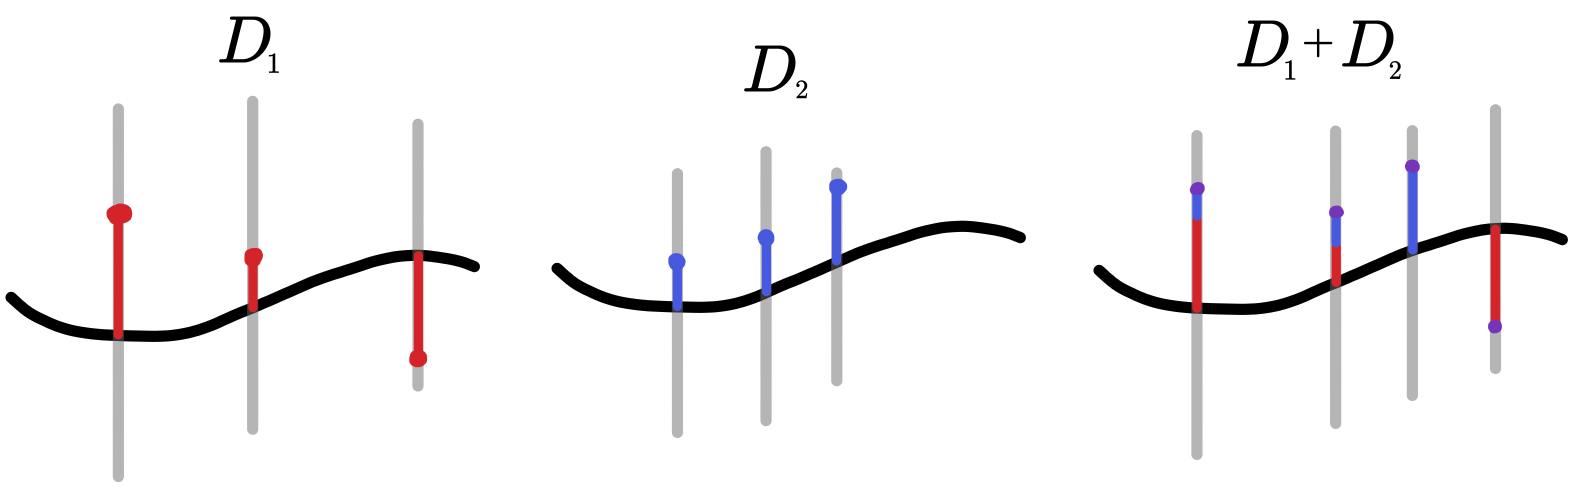
\includegraphics[width=\textwidth]{divisors}
  \caption{Visualising divisors and their sums}
\end{figure}
I will now define the \emph{degree} of a divisor and an order relation on
the group of divisors. The degree of a divisor $D$ is simply the integer
\[
  \deg(D) = \sum_{P\in X} D(P).
\]
Next, I say $D$ is \emph{effective} and write $D\geq 0$ if $D(P)\geq 0$
for all $P\in X$. Then, given two divisors $D, D^{\prime}$, I can define
$D\geq D^{\prime}$ if the divisor $D-D^{\prime}$ is effective.

Important types of divisors are the ones associated to a non-zero rational
function $f\in k(X)^{\times}$. For a point $P\in X$, the ring
$\mathscr{O}_{X,P}$ is a discrete valuation ring (DVR) with valuation
$\ord_{P}$. Then, the divisor of $f$ is defined as follows.
\[
  (f) = \sum_{P\in X}\ord_{P}(f)P.
\]
\begin{ex}
  Consider $X=\mathbb{P}^{1}$ and
  \[f(X_{0}, X_{1})=\frac{X_{1}-X_{0}}{X_{1}}\in k(\mathbb{P}^{1}).\]
  Since $f(X_{0}, X_{1})$ is a unit in the the local rings
  $\mathscr{O}_{X,P}$ for $P\neq [1:0], [1:1]$, we have $\ord_{P}(f)=0$
  at those points $P$. The points $[1:0]$ and $[1:1]$ are contained in the
  affine piece $\mathbb{A}_{0}^{1}=\Set{[X_{0},X_{1}]\in\mathbb{P}^{1}\mid
    X_{0}\neq 0}$. The dehomogenised version of $f$ on $\mathbb{A}_{0}^{1}$ is
  given by $f(x)=\frac{x-1}x$. One can immediately see that
  $\ord_{P_{0}}(f)=-1$ for $P_{0}=[1:0]$ and $\ord_{P_{1}}(f)=1$ for
  $P_{1}=[1:1]$. Therefore,
  \[(f)=P_{1}-P_{0}.\]
\end{ex}
\begin{rem}
  The divisor of a rational function should be thought of as counting the
  orders of zeros and poles of the function.
\end{rem}
It is useful to consider a non-constant element $f$ of $k(X)$ as a morphism
$f:X\to\mathbb{P}^{1}_{k}$. Note that $f$ induces an inclusion
$k\left(\mathbb{P}^{1}_{k}\right)\subseteq k\left(X\right)$ of function
fields. This fact can be used to define a homomorphism
$f^{\ast}:\Div\left(\mathbb{P}^{1}_{k}\right)\to\Div\left(X\right)$ in the
following way \cite{hartshorne}. Firstly, suppose $Q$ is a point of
$\mathbb{P}^{1}_{k}$ and let $t$ be a local uniformiser of
$\mathscr{O}_{\mathbb{P}^{1},Q}$. Then, one defines
\[
  f^{\ast}(Q)=\sum_{f(P)=Q}\ord_{P}(t)\,P.
\]
This definition is independent of the choise of local uniformiser: Suppose
$t^{\prime}$ is another local uniformiser of $\mathscr{O}_{\mathbb{P}^{1},Q}$.
Then, there is a unit $u$ of $\mathscr{O}_{X,Q}$ such that $t^{\prime}=ut$. If
$P\in X$ is a point such that $f(P)=Q$, then $u$ is a unit of
$\mathscr{O}_{X,P}$. Thus, $\ord_{P}(t)=\ord_{P}(t^{\prime})$. Furthermore, this
definition can be linearly extended for an arbitrary divisor
$D\in\Div(\mathbb{P}^{1}_{k})$. Now, the following lemma will be useful.
\begin{lemm}\label{lemm:deg_of_induced}
  If $f\in k(X)$, then for the induced morphism $f^{\ast}:\Div\left(
    \mathbb{P}^{1}_{k}\right)\to\Div\left(X\right)$ we have
  \[
    \deg\left(f^{\ast}(D)\right)=[k(X):k(\mathbb{P}^{1}_{k})]\,\deg(D).
  \]
\end{lemm}
\begin{proof}
  See Proposition 6.9 of \cite{hartshorne} chapter II.
\end{proof}
\begin{cor}\label{cor:rational_deg_zero}
  Suppose $f\in k(X)^{\times}$. Then, $\deg\left((f)\right)=0$.
\end{cor}
\begin{proof}
  If $f$ is a constant, then the statement is immediate. Thus, assume
  $f$ is not a constant. Then, one can write
  $(f)=f^{\ast}(0)-f^{\ast}(\infty)$ and compute the degree:
  \[
    \deg\left((f)\right)=\deg(f^{\ast}(0))-\deg(f^{\ast}(\infty))
    =[k(X):k(\mathbb{P}^{1}_{k})]-[k(X):k(\mathbb{P}^{1}_{k})]=0.
  \]
\end{proof}
\begin{rem}
  Note that divisors of rational functions form a group since
  $(f)+(g)=(fg)$. Then, we can take the quotient of $\Div X$ by this group.
  The quotient is called the Picard group $\Pic X$ and its elements are
  called \textbf{divisor classes}. Thus, there is an equivalence relation on
  $\Div X$ such that
  \[
    D\sim D^{\prime}\iff \exists f\in k(X)^{\times},\ D^{\prime}=D+(f).
  \]
  Then, $D$ and $D^{\prime}$ are said to be \textbf{linearly equivalent}.
\end{rem}

Now, say I want to control the ``order of vanishing'' of a rational function
$f\in k(X)^{\times}$ at the points of the curve $X$. For example, if I want
$f$ to have a ``pole'' only at some point $P\in X$ with order at least $-2$,
I can express this requirement in the following way. Define a divisor
$D=-2P$. Then, I require that $(f)\geq D$. Conventionally, we would actually
set $D=2P$ and require that $(f)\geq -D$. This motivates us to define the
sheaf $\mathcal{L}(D)$ of such functions:
\[
  \left(\mathcal{L}(D)\right)(U)=\Set{f\in k(X)\mid
  \forall P\in U,\ \ord_{P}(f)\geq -D(P)}
\]
\begin{figure}[H]
  \centering
  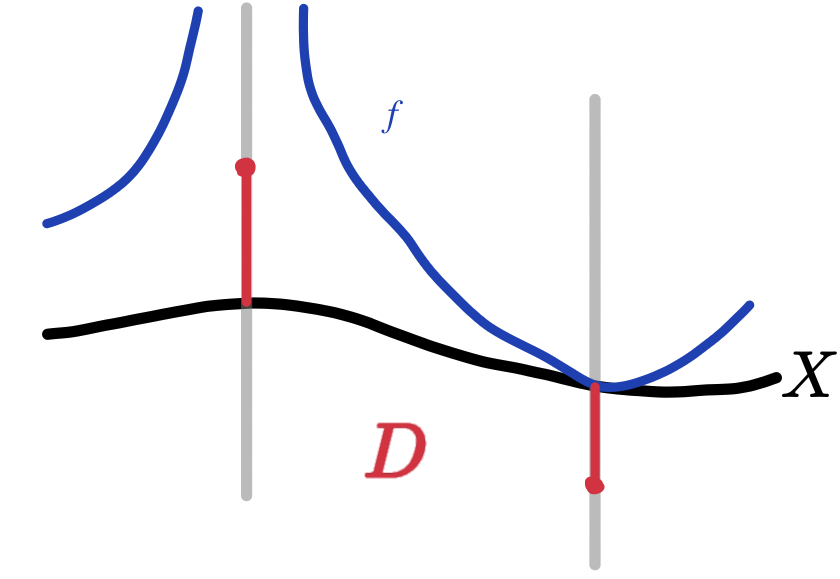
\includegraphics[width=.6\textwidth]{divisor_section}
  \caption{A section of the sheaf $\mathcal{L}(D)$}
\end{figure}
\begin{prop}
  The sheaves $\mathcal{L}(D)$ are quasi-coherent for every divisor $D$.
\end{prop}
\begin{proof}
  Firstly, $\mathcal{L}(D)$ is clearly a sheaf of $\mathscr{O}_{X}$-modules:
  If $f, g\in\mathcal{L}(D)(U)$, then it is clear that
  \[
    \forall P\in U,\ \ord_{P}(f+g)\geq -D(P).
  \]
  Moreover, if $h\in\mathscr{O}_{X}(U)$, then multiplying $f$ by $h$ only
  increases the order at all points, since $\ord_{P}(h)$ is never negative
  on $U$.

  Now, suppose $U\subseteq X$ is an affine open set and let $P\in U$ be a
  point where $D$ is non-zero. Then, take the open set
  $U_{P}^{\prime}\subseteq U$, which doesn't contain any of the other points
  where $D$ is non-zero. One can find a function $\phi_{P}\in k(X)$ in some
  neighbourhood $U_{P}\subseteq U_{P}^{\prime}$ of $P$ such that $(\phi_{P})=P$
  (by Lemma 7.5.6 in \cite{gathmann}). Now, multiplication by $\phi_{P}$
  defines an isomorphism $\mathcal{L}(D)(U_{P})\to \mathscr{O}_{U_{P}}$.
  Since quasi-coherence can be checked locally, this finishes the proof.
\end{proof}
The following proposition will also be useful later.
\begin{prop}\label{prop:global_sec_negative_divisor}
  If a divisor $D$ has negative degree, then $H^{0}(X,\mathcal{L}(D))=0$.
\end{prop}
\begin{proof}
  Suppose $f\in H^{0}(X,\mathcal{L}(D))$. Then, $(f)\geq -D$
  so that $\deg((f))\geq -\deg(D)$, but this implies $\deg(D)\geq 0$
  by Prop.~\ref{cor:rational_deg_zero}. This contradicts the assumption on
  $D$.
\end{proof}

I will now turn to discussing differentials. In geometry, spaces are often
studied locally by looking at their tangent spaces. But the notion of
the tangent space does not translate directly to algebraic geometry,
and we would like to have a more algebraic alternative. It turns out that it
is easier to give an algebraic definition of the \emph{cotangent space},
the dual space of the tangent space. The cotangent space can be defined
abstractly as a module of differentials, which are nice to work with from
an algebraic perspective. I will not attempt to make the connection to
geometry more apparent since giving geometric motivation for the definitions
would take us too far from the focus of the article, and thus I leave it out.
For a soft exposition of differential forms in analysis, I recommend reading
Terence Tao's excellent article \cite{tao}.
\begin{defin}
  For a commutative algebra $F$ over the field $k$, the module of
  $k$-differentials of $F$ is the free $F$-module $\Omega(F)$ generated
  by the symbols $df$ for $f\in F$ with the following rules.
  \begin{itemize}
    \item $d(f+g)=df+dg$ for $f, g\in F$,
    \item $d(fg)=f\,dg+g\,df$ for $f, g\in F$,
    \item $da = 0$ for $a\in k$.
  \end{itemize}
\end{defin}
Note that this definition implies that the differential map $d:F\to\Omega(F)$
is $k$-linear: $d(af)=a\,df+f\,da=a\,df$ for $a\in k$. I will write
$\Omega$ for the module $\Omega\left(k(X)\right)$.
\begin{prop}
  Suppose $t$ is a local uniformiser of $\mathscr{O}_{X,P}$ at some
  point $P\in X$. Then, $\Omega$ is spanned by the differential $dt$.
\end{prop}
\begin{proof}
  First, consider the $k$-vector space
  $\Omega\left(\mathscr{O}_{X,P}\right)/\mathfrak{m}_{P}\Omega\left(
    \mathscr{O}_{X,P}\right)$, where
  $\mathfrak{m}_{P}$ is the maximal ideal of $\mathscr{O}_{X,P}$. I will show
  that this space is spanned by the differential $dt$ and then apply
  Nakayama's lemma. Thus, take an element $\sum f_{i}\,dg_{i}\in\Omega\left(
    \mathscr{O}_{X,P}\right)$. As $\mathscr{O}_{X,P}/\mathfrak{m}_{P}=k$,
  one can write
  \[
    f_{i}=m_{i}+a_{i}\text{ and }g_{i}=m_{i}^{\prime}+a_{i}^{\prime}
    \text{, where } m_{i}, m_{i}^{\prime}\in\mathfrak{m}_{P}
    \text{ and } a_{i}, a_{i}^{\prime}\in k.
  \]
  Then, $f_{i}\,dg_{i}\equiv a_{i}\,dg_{i}$ modulo
  $\mathfrak{m}_{P}\Omega\left(\mathscr{O}_{X,P}\right)$.
  Furthermore, since $\mathfrak{m}_{P}=(t)$, there is
  $r_{i}\in\mathscr{O}_{X,P}$ such that $m_{i}^{\prime}=r_{i}t$. One can again
  write $r_{i}=m_{i}^{\prime\prime}+a_{i}^{\prime\prime}$ so that
  $m_{i}^{\prime}=a_{i}^{\prime\prime}t+m_{i}^{\prime\prime}t$. Therefore,
  \[
    dg_{i}=d\left(m_{i}^{\prime}+a_{i}^{\prime}\right)=dm_{i}^{\prime}
    =a_{i}^{\prime\prime}\,dt+m_{i}^{\prime\prime}\,dt+t\,dm_{i}^{\prime\prime}
    \equiv a_{i}^{\prime\prime}\,dt.
  \]
  and thus
  \[
    \sum f_{i}\,dg_{i}\equiv \sum a_{i}a_{i}^{\prime\prime}\,dt.
  \]
  Since I have shown that $dt$ forms a basis of
  $\Omega\left(\mathscr{O}_{X,P}\right)/\mathfrak{m}_{P}\Omega\left(
    \mathscr{O}_{X,P}\right)$, I can apply Nakayama's lemma
  (see Proposition 2.8 in \cite{am}), which implies that $dt$ also generates
  $\Omega\left(\mathscr{O}_{X,P}\right)$ as a $\mathscr{O}_{X,P}$-module.
  Now, suppose $f\in k(X)$. Such a function has an expansion
  \[
    f=a_{-n}t^{-n}+a_{-n+1}t^{-n+1}+\cdots +a_{-1}t^{-1}+ut^{n},
  \]
  where $a_{i}\in k$, $u$ is a unit in $\mathscr{O}_{X,P}$ and $n\geq 0$.
  Then,
  \[
    df=-na_{-n}t^{-n-1}\,dt+\cdots-a_{-1}t^{-2}\,dt+d\left(ut^{n}\right)
  \]
  Since $ut^{n}\in\mathscr{O}_{X,P}$, the differential $df$ is in the span
  of $dt$. It is easy to see that the statement follows from here.
\end{proof}
This proposition lets us to define the order of a differential
$\omega\in\Omega$ as follows. Write $\omega=f\,dt$ for $f\in k(X)$. Then,
\[
  \ord_{P}(\omega)=\ord_{P}(f).
\]
Now, one can define the divisor $(\omega)$ of $\omega$ in the same way as
the divisor of a rational function:
\[
  (\omega)=\sum_{P\in X}\ord_{P}(\omega)P.
\]
It turns out that divisors of this kind are all linearly equivalent: suppose
$\omega_{1}=f_{1}\,dt$ and $\omega_{2}=f_{2}\,dt$. Then,
\[
  \omega_{1}=\frac{f_{1}}{f_{2}}\, f_{2}\,dt=\frac{f_{1}}{f_{2}}\omega_{2}
  \implies (\omega_{1})=\left(\frac{f_{1}}{f_{2}}\right)(\omega_{2}).
\]
Thus, the divisors of differentials lie in the same divisor class called the
\emph{canonical class}. A representative of the class is called the
\emph{canonical divisor} $K_{X}$.

Next I define a module of differentials related to a divisor $D$
on $X$ in the same way as we defined the sheaf $\mathcal{L}(D)$:
\[
  \Omega(D)=\Set{\omega\in\Omega\mid \forall P\in X,\ \ord_{P}(\omega)
  \geq D(P)}.
\]
(in the modern literature one requires $\ord_{P}(\omega)\geq -D(P)$
to match the definition of $\mathcal{L}(D)$, but here I follow \cite{serre}
with the notation). Lastly, I will define the \emph{residue} of a
differential, which will be the main ingredient in the proof of Serre
duality in the next section.
\begin{defin}
  Let $\omega=f\,dt\in\Omega$, where $t$ is a local uniformiser of
  $\mathscr{O}_{X,P}$ for some point $P\in X$. Then, $f$ can be embedded
  in the ring $k((t))$ of formal series over $k$, where it has a series
  expansion in terms of $t$:
  \[
    f=\sum_{i\geq n}a_{i}t^{i},
  \]
  where $n\in\mathbb{Z}$ and $a_{i}\in k$. Then, the residue of $\omega$
  at $P$ is defined as $\res_{P}(\omega)=a_{-1}$.
\end{defin}
A priori, this definition depends on the local uniformiser $t$, and thus
I need to show that the definition is indeed independent of the choise
of a local uniformiser. I will only give a proof sketch, but a more detailed
proof can be found in \cite{serre}.
\begin{lemm}\label{lemm:res_quotient}
  For a non-zero function $f$, we have $\res_{P}(df/f)=\ord_{P}(f)$.
\end{lemm}
\begin{proof}
  If $t$ is a local uniformiser of $\mathscr{O}_{X,P}$, then $f$ can be
  written as $f=ut^{n}$, where $n=\ord_{P}(f)$. Then,
  \[
    df/f = \frac{t^{n}\,du + nut^{n-1}\,dt}{ut^{n}}=du/u+n\,dt/t.
  \]
  Thus, $\res_{P}(df/f)=\res_{t}(du/u)+n$, but since $u$ is a unit in
  $\mathscr{O}_{X,P}$, the residue $\res_{t}(du/u)$ is clearly zero.
\end{proof}
\begin{prop}
  Fix a point $P\in X$ and let $t$ and $r$ be two local uniformisers of
  $\mathscr{O}_{X,P}$. Denote by $\res_{t}$ and $\res_{r}$ the function
  $\res_{P}$ calculated using $t$ and $r$ respectively. Then,
  $\res_{t}(\omega)=\res_{r}(\omega)$ for all differentials $\omega\in\Omega$.
\end{prop}
\begin{proof}[Proof sketch]
  Suppose $f\in k(X)$ is a rational function with a series expansion
  \[
    f=\sum_{i\geq n}a_{i}t^{i},
  \]
  in $t$. Then, it is possible to construct a module of differentials, where
  \[
    df=\left(\sum_{i\geq n}ia_{i}t^{i-1}\right)\,dt.
  \]
  This is probably the most non-trivial statement of the proof, and the
  construction can be found in \cite{serre}. Now, we can write a
  differential $\omega$ in this module as
  \[
    \omega = \sum_{n\geq 0}a_{n}\,du/u^{n}+\omega_{0},
  \]
  where $\omega_{0}$ is a differential with $\ord_{P}(\omega_{0})\geq 0$.
  Then, $\res_{u}(\omega)=a_{1}$ and $\res_{t}(\omega)=
  \sum a_{n}\res_{t}(du/u^{n})$. Now, consentrate first on the term
  $a_{1}\res_{t}(du/u)$. I can apply Lemma~\ref{lemm:res_quotient}
  to get $\res_{t}(du/u)=\ord_{P}(u)=1$. Therefore,
  \[
    \res_{t}(\omega) = a_{1}+\sum_{n>0}\res_{t}(du/u^{n}).
  \]
  Hence, it is enough to show that $\res_{t}(du/u^{n})=0$ for $n>0$.

  In characteristic zero, we can write
  \[
    du/u^{n}=d\left(-\frac1{(n-1)u^{n-1}}\right).
  \]
  But this immediately implies that $\res_{t}(du/u^{n})=0$ since
  differentiating a series can never result in a term of the form
  $a_{-1}t^{-1}$. The proof for positive characteristic follows from the
  statement in zero characteristic and can be found in \cite{serre}.
\end{proof}
Now, I will prove the \emph{residue theorem}, which is used in the proof
of the Serre duality theorem.
\begin{thm}[Residue Theorem]\label{thm:residue_theorem}
  For every differential $\omega\in\Omega$, we have that
  \[
    \sum_{P\in X}\res_{P}(\omega)=0.
  \]
\end{thm}
First I prove the theorem for the case when $X=\mathbb{P}^{1}_{k}$.
\begin{lemm}
  The residue theorem holds for $X=\mathbb{P}^{1}_{k}$.
\end{lemm}
\begin{proof}
  Fix a differential $\omega=f\,dt$ on $X$. For convenience, I work with
  dehomogenised representation, and take $f$ to be a rational function
  in one variable $t$. This function has a partial fractions decomposition,
  which is a linear combination of terms of the form listed below. I will
  consider each type separately.
  \begin{description}[style=nextline]
    \item[Term of type $\omega=t^{n}\,dt$:] There are no poles at finite
          points, so the only pole could be at infinity. Changing to
          $u=1/t$, we have $dt=-u^{-2}\,du$ and
          \[\omega=(u^{-n})(-u^{-2}\,du)=\frac{du}{u^{n+2}}.\]
          Then, the residue clearly vanishes: $\res_{\infty}(\omega)=0$.
    \item[Term of type $\omega=\frac{dt}{t-a}$:] Clearly $\res_{a}(\omega)=1$,
          and there are no other poles at finite points. But there is also a
          pole at infinity. Again, changing to $u=1/t$, we get
          \begin{align*}
            f(u)&=\left(\frac{u}{1-au}\right)(-u^{-2}\,du)
            =-\frac1{u}\cdot\frac1{1-au}\,du \\
            &=-\frac1{u}\left(1+au+(au)^{2}+\cdots\right)\,du.
          \end{align*}
          Therefore, $\res_{a}(\omega)=-1$ and the residues of the two points
          cancel.
    \item[Term of type $\omega=\frac{dt}{(t-a)^{n}}$ for $n>1$:] Following
          a similar argument as above, one can check that in this case
          the residue is zero also at $a$ and $\infty$.
  \end{description}
\end{proof}
Let $X$ be a curve as before. Again, a non-constant function $\phi\in k(X)$
induces an embedding $k(\mathbb{P}^{1}_{k})\hookrightarrow k(X)$, and I hope
to use this embedding to apply the above lemma in the case of an arbitrary
curve $X$. Now, one can consider the trace map $\tr_{k(X)/k(\mathbb{P}^{1}_{k})}$
defined as follows \cite{milne}. Multiplication by an element
$\alpha\in k(X)$ defines a $k(\mathbb{P}^{1}_{k})$-linear map
$\alpha^{\ast}: E\to E: x\mapsto \alpha x$. Then, we simply define
$\tr_{k(X)/k(\mathbb{P}^{1}_{k})}(\alpha)$ to be the usual trace of this linear
transformation $\alpha^{\ast}$. Next I translate this definition to
differentials on $k(X)$. We can write any differential
$\omega\in\Omega(k(X))$ as $\omega=f\,d\phi$. Then, one can make the
following definition.
\[
  \tr:\Omega(k(X))\to \Omega(k(\mathbb{P}^{1}_{k}))
  :f\,d\phi\mapsto \left(\tr_{k(X)/k(\mathbb{P}^{1}_{k})}(f)\right)\,d\phi
\]
Finally, the residue formula is implied by the following lemma which
is proved in \cite{serre}.
\begin{lemm}
  For every point $P\in\mathbb{P}^{1}_{k}$, we have
  \[
    \sum_{Q\in\phi^{-1}(P)}\res_{Q}(\omega)=\res_{P}(\tr(\omega)).
  \]
\end{lemm}

\subsection{Proof of Riemann-Roch}
I am now able to state and prove an ``incomplete'' version of the
Riemann-Roch theorem, which I will make complete after proving Serre
duality.

\begin{thm}[Riemann-Roch, cohomology version]
  \label{thm:riemann_roch_cohomology}
  For every divisor $D$,
  \[
    h^{0}(X, \mathcal{L}(D))-h^{1}(X, \mathcal{L}(D))=\deg(D)+1-g,
  \]
  where $g=h^{1}(X, \mathscr{O}_{X})$.
\end{thm}
\begin{proof}
  One can use an induction argument, because any divisor $D$ can be
  obtained from the zero divisor by adding and subtracting points.
  Thus, I proceed by first proving the base case and then proving
  the induction step.

  \begin{description}[style=nextline]
    \item[base case$\big)$]
          Since $\mathcal{L}(0)=\mathscr{O}_{X}$ and $\deg(0)=0$,
          I need to verify that
          \[h^{0}(X, \mathscr{O}_{X})-h^{1}(X, \mathscr{O}_{X})=1-g.\]
          But note that the only globally defined regular functions
          on $X$ are constant and thus they form a one-dimensional vector
          space. Moreover, $h^{1}(X, \mathscr{O}_{X})=g$ by definition
          so that the equality holds.
    \item[induction step$\big)$]
          In the induction step I want to relate the 0th and the 1st
          cohomology groups of $\mathcal{L}(D)$ to the 0th and
          1st cohomology groups of $\mathcal{L}(D+P)$, where
          $P$ is some point. To do this, first note that
          $\mathcal{L}(D)$ is a subsheaf of $\mathcal{L}(D+P)$, since
          the orders of the sections of $\mathcal{L}(D+P)$ at $P$ are
          allowed to be smaller than the orders of the sections of
          $\mathcal{L}(D)$ at $P$. Thus, there is an exact sequence
          \[
          \begin{tikzcd}
            0\arrow{r} & \mathcal{L}(D)\arrow{r} & \mathcal{L}(D+P)\arrow{r}
            & Q\arrow{r} & 0,
          \end{tikzcd}
          \]
          where $Q$ is the quotient sheaf. The stalks of $Q$ are clearly
          zero away from $P$. The stalk at $P$ consists of zero and
          elements of the form $u/t^{n+1}$, where $t$ is the local
          uniformiser of $\mathscr{O}_{X,P}$, $u$ is a unit in
          $\mathcal{O}_{X,P}$, and $n$ is the order of $P$ in $D$.
          As $\mathcal{O}_{X,P}/(t)=k$, we can write $u=vt+r$,
          where $v\in\mathcal{O}_{X,P}$ and $r\in k$.
          Then,
          \[\frac{u}{t^{n+1}}=\frac{v}{t^n}+\frac{r}{t^{n+1}}.\]
          Since $v/t^n$ is an element of $\mathcal{L}(D)_{P}$, we conclude
          that every element of $\mathcal{L}(D+P)_{P}$ is equivalent to
          an element $r/t^{n+1}$ modulo $\mathcal{L}(D)_{P}$ for some
          $r\in k$. Therefore, $Q_{P}\cong k$ and $Q$ is the skyscraper sheaf
          $k_{P}$.

          Now we apply our cohomology machinery on the SES
          \[
          \begin{tikzcd}
            0\arrow{r} & \mathcal{L}(D)\arrow{r} & \mathcal{L}(D+P)\arrow{r}
            & k_{P}\arrow{r} & 0
          \end{tikzcd}
          \]
          to get the following exact sequence (using
          Prop.~\ref{prop:sky_cohom}).
          \[
          \begin{tikzcd}
            0\arrow{r} & H^{0}(X, \mathcal{L}(D))\arrow{r}
            & H^{0}(X, \mathcal{L}(D+P))\arrow{r}
            & H^{0}(X, k_{P}) \\
            \arrow{r} & H^{1}(X, \mathcal{L}(D))\arrow{r}
            & H^{1}(X, \mathcal{L}(D+P))\arrow{r} & 0.
          \end{tikzcd}
          \]
          Now, this exact sequence of vector spaces implies the following
          equality.
          \[
          h^{0}(X,\mathcal{L}(D))-h^{0}(X, \mathcal{L}(D+P))
          +1-h^{1}(X,\mathcal{L}(D))+h^{1}(X,\mathcal{L}(D+P)) = 0.
          \]
          Therefore,
          \begin{align*}
            h^{0}(X,\mathcal{L}(D+P))&-h^{1}(X,\mathcal{L}(D+P))
            =\left(h^{0}(X,\mathcal{L}(D))-h^{1}(X,\mathcal{L}(D+P))\right)
              +1 \\
            =&\deg(D)+1-g+1\quad\text{(by induction hypothesis)} \\
            =&\deg(D+P)+1-g.
          \end{align*}
          This is exactly the induction step we wanted to prove.
          We also need to prove
          \[
            h^{0}(X,\mathcal{L}(D-P))-h^{1}(X,\mathcal{L}(D-P))
            =\deg(D-P)+1-g,
          \]
          but we can run the same argument starting with the SES
          \[
          \begin{tikzcd}
            0\arrow{r} & \mathcal{L}(D-P)\arrow{r} & \mathcal{L}(D)\arrow{r}
            & k_{P}\arrow{r} & 0.
          \end{tikzcd}
          \]
  \end{description}
\end{proof}
\begin{lwarn}
  One would need to also prove that the cohomology groups are finite
  dimensional to begin with. The details can be found in \cite{serre}.
\end{lwarn}

This form of the theorem is not the most useful one for applications,
because computing $h^{1}(X,\mathcal{L}(D))$ is not easy. However, one can
get a nice expression for this space using the Serre Duality theorem, which
I will prove in the next section:
\newtheorem*{thm:serre}{Theorem~\ref{thm:serre}}
\begin{thm:serre}[Serre Duality]
  If $X$ is an algebraic curve as before
  and $D$ is a divisor on $X$, there is an isomorphism
  \[
    \dual{D}\cong \diffs{D}.
  \]
  of $k$-vector spaces.
\end{thm:serre}
Since we are only interested in the dimension of $h^{1}(X,\mathcal{L}(D))$,
I will use the following lemma to give the dimension in terms of the
canonical divisor.
\begin{lemm}\label{lemm:diffs_dim}
  We have the following equality in dimensions.
  \[\dim\left(\Omega(D)\right)=h^{0}(X,\mathcal{L}(K_{X}-D))\]
\end{lemm}
\begin{proof}
  Write $K_{X}=(\omega_{0})$ with $\omega_{0}=f_{0}\,dt$ and fix a
  differential $\omega=f\,dt$. Then, $\omega=\frac{f}{f_{0}}\omega_{0}$
  and we have
  \[
    \omega\in\Omega(D)\iff (\omega)\geq D
    \iff\left(\frac{f}{f_{0}}\right)+(\omega_{0})\geq D\iff
    \frac{f}{f_{0}}\in H^{0}(X,\mathcal{L}(K_{X}-D)).
  \]
  In other words, the elements of $H^{0}(X,\mathcal{L}(K_{X}-D))$ are in
  bijection with the elements of $\Omega(D)\cong\dual{D}$.
\end{proof}
Now, this equality lets us write the ``complete'' form of the Riemann-Roch
theorem.
\begin{thm}[Riemann-Roch]\label{thm:riemann_roch}
  For every divisor $D$,
  \[
    h^{0}(X, \mathcal{L}(D))-h^{0}(X, \mathcal{L}(K_{X}-D))=\deg(D)+1-g,
  \]
  where $g=h^{1}(X, \mathscr{O}_{X})$.
\end{thm}

%\subsection{Applications to the classification of curves}
%Before proving the Serre duality theorem, I want to take some time to
%look at applications of the Riemann-Roch theorem.
\subsection{An application to the classification of curves}
Before proving the Serre duality theorem, I want to take some time to
look at an application of the Riemann-Roch theorem using \cite{hartshorne}
as my source. A major project in algebraic geometry is to give a
classification of different algebraic varieties. The Riemann-Roch theorem
helps us prove statements about varieties based solely on topological data,
namely the genus of the curve. First, I give a formula for the degree
of the canonical divisor on a curve.
\begin{lemm}
  The degree of the canonical divisor $K_{X}$ is $2g-2$, where $g$ is the
  genus of $X$.
\end{lemm}
\begin{proof}
  Set $D=K_{X}$ so that the Riemann-Roch theorem yields
  \begin{align*}
    h^{0}(X,\mathcal{L}(K_{X}))-h^{0}(X,\mathscr{O}_{X})&=\deg(D)+1-g \\
    h^{1}(X,\mathscr{O}_{X})-1&=\deg(D)+1-g \\
    2g-2&=\deg(D),
  \end{align*}
  where $h^{0}(X,\mathcal{L}(K_{X}))=h^{1}(X,\mathscr{O}_{X})$ is given
  by the Serre duality theorem.
\end{proof}
Now I can give a classification of curves of genus 0.
\begin{thm}
  Any curve $X$ of genus 0 is isomorphic to $\mathbb{P}^{1}_{k}$.
\end{thm}
\begin{proof}
  Fix two point $P,Q\in X$ and consider the divisor $D=P-Q$. The Riemann-Roch
  theorem implies
  \[
    h^{0}(X,\mathcal{L}(D))-h^{0}(X,\mathcal{L}(K_{X}-D))
    =\deg(D)+1=1.
  \]
  Note that $\deg(K_{X}-D)=-2-0=-2<0$ by the above lemma. Thus,
  \[
    h^{0}(X,\mathcal{L}(K_{X}-D))=0
  \]
  by Prop.~\ref{prop:global_sec_negative_divisor} and hence, the space
  $H^{0}(X,\mathcal{L}(D))$ is non-empty. Now, let
  $f\in H^{0}(X,\mathcal{L}(D))$. Then, there is an effective divisor
  $D^{\prime}$ on $X$ such that $D^{\prime}=(f)+D$. Then, we have
  $\deg\left(D^{\prime}\right)=\deg\left((f)\right)+\deg\left(D\right)=0$.
  But the only effective divisor with degree 0 is the zero divisor.
  Therefore, $(f)=Q-P$. One can see that $f^{\ast}(0)=Q$, where
  $f^{\ast}$ is the homomorphism induced by $f$. Applying
  Lemma~\ref{lemm:deg_of_induced}, we get the following.
  \begin{align*}
    [k(X):k(\mathbb{P}^{1})]\cdot 1
    &=\deg\left(f^{\ast}(0)\right) \\
    &=\deg(Q) = 1.
  \end{align*}
  Therefore, the function fields $k(X)$ and $k\left(\mathbb{P}^{1}_{k}\right)$
  are isomorphic. Since $X$ and $\mathbb{P}^{1}_{k}$ are non-singular,
  it follows by Proposition 6.7 in \cite{hartshorne} that the two curves
  are isomorphic.
\end{proof}

\section{Serre duality}
The rest of this paper is devoted to proving the Serre duality:
\newtheorem*{thm:serre}{Theorem~\ref{thm:serre}}
\begin{thm:serre}[Serre Duality]
  If $X$ is an algebraic curve as in the previous section
  and $D$ is a divisor on $X$, there is an isomorphism
  \[
    \dual{D}\cong \diffs{D}.
  \]
  of $k$-vector spaces.
\end{thm:serre}
I will prove the theorem by first finding a more concrete representation of
$H^{1}(X,\mathcal{L}(D))$ and then constructing a perfect pairing between
$H^{1}(X,\mathcal{L}(D))$ and $\diffs{D}$,
which will give us the isomorphism.

\subsection{Concrete representation of $H^{1}(X,\mathcal{L}(D))$}
To prove the Serre duality, we do not want to directly work with the \v Cech
cohomology definition of $H^{1}(X,\mathcal{L}(D))$.
Instead we want to give a more concrete description of
$H^{1}(X,\mathcal{L}(D))$ by finding some SES involving $\mathcal{L}(D)$
and then taking the cohomology sequence of the SES. Since $\mathcal{L}(D)$ is
a subsheaf of the constant sheaf $\underline{k(X)}$, we can simply consider
the following SES.
\[
  \begin{tikzcd}
    0\rar & \mathcal{L}(D)\rar & \underline{k(X)}\rar
    & \underline{k(X)}/\mathcal{L}(D)\rar & 0,
  \end{tikzcd}
\]
which yields the following exact sequence
\[
  \begin{tikzcd}
    H^{0}(X,\underline{k(X)})\rar & H^{0}(X,\underline{k(X)}
    /\mathcal{L}(D))\rar & H^{1}(X,\mathcal{L}(D))\rar
    & H^{1}(X,\underline{k(X)}).
  \end{tikzcd}
\]
But Prop.~\ref{prop:const_sheaf} implies that
$H^{0}(X,\underline{k(X)})=k(X)$ and $H^{1}(X,\underline{k(X)})=0$
so that the exact sequence simplifies to
\begin{equation}\label{eq:repartition_ses}
  \begin{tikzcd}
    k(X)\rar & H^{0}(X,\underline{k(X)}/\mathcal{L}(D))\rar
    & H^{1}(X,\mathcal{L}(D))\rar & 0.
  \end{tikzcd}
\end{equation}
Let us first try to understand the space
$H^{0}(X,\underline{k(X)}/\mathcal{L}(D))$. An element of the space
is of the form $([f_{P}])_{P\in X}$, where $[f_{P}]$ is the equivalence
class of some $f_{P}\in k(X)$ modulo $\mathcal{L}(D)_{P}$.
These elements are actually quite simple, because one can show that the
components $[f_{P}]$ are zero almost everywhere.
% TODO: Add picture with curve X and section f \in H^0(X,k(X)/L(D)) above it.
In other words, we can write $H^{0}(X,\underline{k(X)}/\mathcal{L}(D))$ as a
direct sum of stalks.
\begin{lemm}
  For a divisor $D$ on a curve $X$, the following equality holds.
  \[
    H^{0}(X,\underline{k(X)}/\mathcal{L}(D))=\bigoplus_{P\in X}
    k(X)/\mathcal{L}(D)_{P}.
  \]
\end{lemm}
\begin{proof}
  I will first show the inclusion in forward direction:
  \[
    H^{0}(X,\underline{k(X)}/\mathcal{L}(D))\subseteq\bigoplus_{P\in X}
    k(X)/\mathcal{L}(D)_{P}.
  \]
  In other words, I need to check that the components $[f_{P}]$ of some
  $([f_{P}])_{P\in X}\in H^{0}(X,\underline{k(X)}/\mathcal{L}(D))$ are non-zero
  for only finitely many $P\in X$. Thus, suppose $([f_{P}])_{P\in X}\in
  H^{0}(X,\underline{k(X)}/\mathcal{L}(D))$. Firstly, the divisor $D$ is
  non-zero only at finitely many points. The components $[f_{P}]$ may or may
  not be zero at those points, but I can ignore those points in any case
  since there are finitely many of them. Thus, assume $P$ is a point where
  $D(P)=0$. At such a point, the stalk $\mathcal{L}(D)_{P}$ is equal to the
  ring of germs with non-negative order at $P$, which is of course the ring
  $\mathscr{O}_{X,P}$. Now, it is a basic result in algebraic geometry that
  a rational function $f\in k(X)$ on a curve $X$ has negative order only
  at finitely many points so that $f_{P}\in\mathscr{O}_{X,P}$ for almost
  all points $P$. Therefore, we see that $[f_{P}]=0$ for almost all points
  $P$.
  % TODO: Insert a picture of the plane with points where the section
  %       might be non-zero.

  Next I show the inclusion in the reverse direction:
  \[
    H^{0}(X,\underline{k(X)}/\mathcal{L}(D))\supseteq\bigoplus_{P\in X}
    k(X)/\mathcal{L}(D)_{P}.
  \]
  Thus, let $([f_{P}]_{P\in X})\in\displaystyle\bigoplus
  k(X)/\mathcal{L}(D)_{P}$. I want to show that the components $[f_{P}]$
  form a global section of $\underline{k(X)}/\mathcal{L}(D)$. Let us
  fix an arbitrary point $P\in X$. I want to find an open neighbourhood
  $U\ni P$ and a section $g\in k(X)$ such that $\forall Q\in U,\ [f_{Q}]=[g]$.
  If I denote by $P_{1},\ldots,P_{r}$ the points where $D$ is non-zero
  and by $Q_{1},\ldots,Q_{s}$ the points where the $f_{Q_{i}}$ have negative
  order, then there are two cases:
  \begin{description}[style=nextline]
    \item[$P\not\in\set{P_{1},\ldots,P_{r},Q_{1},\ldots,Q_{s}}\big)$]
          Since $P$ is none of the points $P_{1},\ldots,P_{r}$,
          $\mathcal{L}(D)_{P}$ consists of all functions $f\in k(X)$
          with non-negative order at $P$: $\ord_{P}(f)\geq 0$.
          Since $P$ is non of the points $Q_{1},\ldots,Q_{s}$,
          $f_{P}\in\mathscr{O}_{X,P}$. Therefore, $f_{P}\in\mathcal{L}(D)_{P}$
          so that $[f_{P}]=[0]$. Now, if we let $U$ be the complement of
          the set $\set{P_{1},\ldots,P_{r},Q_{1},\ldots,Q_{s}}$, we see
          that $[f_{Q}]=[0]$ for every $r_{Q}$ on $U$ so that we can simply
          choose $0\in k(X)$ as the section on the open neighbourhood $U$.
    \item[$P\in\set{P_{1},\ldots,P_{r},Q_{1},\ldots,Q_{s}}\big)$]
          First, denote $Y=\set{P_{1},\ldots,P_{r},Q_{1},\ldots,Q_{s}}
          \setminus \set{P}$ and $g=f_{P}\in k(X)$. Next, let
          $S_{1},\ldots,S_{t}$ be the points where the $g_{S_{i}}$ have
          negative order. Then, let $U$ be the complement of
          $Y\cup \set{S_{1},\ldots,S_{t}}$. As above, $[f_{Q}]=[0]$ for all
          $Q\in U$ except for $Q=P$. But since the points $S_{i}$ are also
          included in the complement, $[g]=[0]$ away from $P$. Thus,
          $[f_{Q}]=[g]$ on $U$.
  \end{description}
\end{proof}
Now, we can express this direct sum in the following way. Consider the
vector space $R$ of families $\{r_{P}\}_{P\in X}$, where $r_{P}\in k(X)$ and
$r_{P}\in\mathscr{O}_{X,P}$ for almost all points $P\in X$.
(Serre calls such a family a \emph{r\'epartition} in \cite{serre}).
Then, define $R(D)=\set{\{r_{P}\}_{P\in X}\mid \ord_{P}(r_{P})\geq -D(P)}$.
It is clear that we have the following isomorphism.
\[
  \bigoplus_{P\in X}k(X)/\mathcal{L}(D)_{P}\cong R/R(D).
\]
Note that r\'epartitions are easier to work with, because the components
$f_{P}$ of some section $(f_{P})_{P\in X}$ of
$\underline{k(X)}/\mathcal{L}(D)$ must be related together so that the
sections satisfy sheaf axioms, whereas there is no such requirement for
r\'epartitions. Therefore, I will make use of r\'epartitions in the rest
of the section.

Now we can return to the SES \eqref{eq:repartition_ses} derived above and
replace $H^{0}(X,\underline{k(X)}/\mathcal{L}(D))$ by $R/R(D)$:
\[
  \begin{tikzcd}
    k(X)\rar & R/R(D)\rar & H^{1}(X,\mathcal{L}(D))\rar & 0.
  \end{tikzcd}
\]
This exact sequence finally gives us the representation of the first
cohomology group: The second map of the sequence is a surjection
onto $H^{1}(X,\mathcal{L}(D))$. The space $k(X)$ can be seen as a subspace
of $R$ and it is thus the kernel of the map. Such a surjection maps $R/R(D)$
onto the space $R\,/\left(R(D)+k(X)\right)$, and thus we get the isomorphism
\[H^{1}(X,\mathcal{L}(D))\cong R/\left(R(D)+k(X)\right).\]
Now, the dual space $\dual{D}$ is simply the space
of linear functionals on $R$, which vanish on $R(D)$ and $k(X)$!

\subsection{Constructing a pairing}
Next I will construct a bilinear form
\[
  \langle -,-\rangle:\diffs{D}\times H^{1}(X,\mathcal{L}(D))\to k.
\]
Note that the space $\diffs{D}$ consists of differential forms $\omega$
such that $(\omega)\geq D$.
%But first we want to understand the space $H^{0}(X,K_{X}
%\otimes\mathcal{L}(D)^{\vee})$ better.
%Consider the stalk of the sheaf
%$K_{X}\otimes\mathcal{L}(D)^{\vee}$ at a point $P$:
%\[
%  \left(K_{X}\otimes\mathcal{L}(D)^{\vee}\right)_{P}
%  =(K_{X})_{P}\otimes_{\mathscr{O}_{X}}\mathcal{L}(D)^{\vee}_{P}
%  =D_{k}(\mathscr{O}_{X})\otimes_{\mathscr{O}_{X}}\mathcal{L}(D)^{\vee}_{P}
%  =D_{k}\left(\mathcal{L}(D)^{\vee}_{P}\right).
%\]
Now, define the bilinear form as follows.
\[
  \langle\omega,r\rangle=\sum_{P\in X}\res_{P}(r_{P}\omega),
\]
where $r=[\{r_{P}\}_{P\in X}]\in R\,/\left(R(D)+k(X)\right)$. I must check
that the map is well-defined: only finitely many terms of the sum can be
non-zero, and its value must be independent of the representation modulo
$R(D)+k(X)$.

Firstly, $\res_{P}(r_{P}\omega)$ can be non-zero only when $P$ is a point
such that $D(P)\neq 0$ or $r_{P}\not\in\mathscr{O}_{X,P}$. Otherwise,
$r_{P},f\in\mathscr{O}_{X,P}$, if we write $\omega=f\,dt$ where $t$ is a
local uniformiser at $P$. This clearly implies that the coefficients of the
terms of negative degree in the series expansion of $r_{P}f$ are all zero.
Secondly, given a repartition $r\in R(D)$, we have $(r_{P}\omega)
=(r_{P})+(\omega) \geq -D+D=0$ and thus $\res_{P}(r_{P}\omega)=0$ by the same
% TODO: Make this part more clear.
argument as above. Also, if $r\in k(X)$, then $\langle \omega,r\rangle=0$ by
the residue theorem (Thm.~\ref{thm:residue_theorem}).

Now, Serre duality will follow if we can show that the map
\[
  \iota_{D}:\diffs{D}\to \dual{D}
  :\omega\mapsto\langle\omega,-\rangle
\]
is a bijection. Every differential $\omega\in\diffs{D}$ is indeed mapped
to elements of $\dual{D}$ since they vanish on $R(D)$ and $k(X)$ by the
arguments in the previous pragraph.

I will proceed to prove the bijectivity of $\iota_{D}$. The proof relies
on the observation that the spaces $\dual{D}$ and $\diffs{D}$ form so called
\emph{filtered families}, which are tied together by $\iota_{D}$. In the
proofs of injectivity and surjectivity we will ``move through the
filtration'' to derive the wanted results. Thus, let us make the following
observation. For any two divisors $D_{1}, D_{2}$ such that $D_{1}\geq D_{2}$,
we have $R(D_{1})\supseteq R(D_{2})$. Therefore, a linear functional
vanishing on $R(D_{1})$ will also vanish on $R(D_{2})$ so that
$H^{1}(X,\mathcal{L}(D_{1}))^{\vee}\subseteq H^{1}(X,\mathcal{L}(D_{2}))^\vee$.
One can also see that if $D_{1}\geq D_{2}$, then $\diffs{D_{1}}
\subseteq\diffs{D_{2}}$. Moreover, these inclusions trivially
commute with $\iota_{\bullet}$ so that the following square is commutative.
\begin{equation}\label{eq:iota_square}
  \begin{tikzcd}[column sep=large]
    \dual{D_{1}}\rar[hook, shorten=.7em, "i_{D_{1}}^{D_{2}}"] & \dual{D_{2}} \\
    \diffs{D_{1}}\uar{\iota_{D_{1}}}\rar[hook]
    & \diffs{D_{2}}\uar["\iota_{D_{2}}"']
  \end{tikzcd}
\end{equation}
\begin{cat}
  The commutativity of this square shows that the maps $\iota_{\bullet}$
  define a natural transformation between the contravariant functors
  \[
    \diffs{-},\dual{-}:\Div(X)\to k\textbf{-Vect},
  \]
  where $\Div(X)$ is the posetal category of divisors on $X$.
  Thus, not only do we get an isomorphism of the vector spaces
  $\diffs{D}$ and $\dual{D}$, but we also get a natural isomorphism
  between the functors $\diffs{-}$ and $\dual{-}$.
\end{cat}

Now, the following lemma will let us ``transport the problem along the
filtration''.
\begin{lemm}\label{lemm:invert_inclusion}
  Suppose $D_{1}$ and $D_{2}$ are two divisors on $X$ such that
  $D_{1}\geq D_{2}$. Furthermore, let $\lambda\in\dual{D_{1}}$ and
  $\omega\in\diffs{D_{2}}$. If $i_{D_{1}}^{D_{2}}(\lambda)
  =\iota_{D_{2}}(\omega)$, then $\omega\in\diffs{D_{1}}$ and
  $\iota_{D_{1}}(\omega)=\lambda$.
\end{lemm}
This lemma is effectively saying that if we can invert $\lambda$
along $\iota_{D_{2}}$, then we can invert it along $\iota_{D_{1}}$, when
$D_{1}\geq D_{2}$.
\begin{proof}
  Assume to the contrary that $\omega\not\in\diffs{D_{1}}$. Then,
  there is a point $P\in X$ such that $\ord_{P}(\omega)<D_{1}(P)$.
  Now we can construct a r\'epartition $r=\{r_{Q}\}_{Q\in X}$ such that
  $r_{Q}=0$ when $Q\neq P$ and $r_{P}=1/t^{\ord_{P}(\omega)+1}$, where $t$ is a
  local uniformiser at $P$. We have $r\in R(D_{1})$, because
  \[
    \ord_{P}(r_{P})=-\ord_{P}(\omega)-1>-D_{1}(P)-1
    \implies \ord_{P}(r_{P})\geq -D_{1}(P).
  \]
  Then,
  \[
    \lambda(r)=i_{D_{1}}^{D_{2}}(r)=\iota_{D_{2}}(\omega)(r)
    =\sum_{Q\in X}\res_{Q}(r_{Q}\omega)=\res_{P}(r_{P}\omega).
  \]
  Since $\ord_{P}(r_{P}\omega)=\ord_{P}(r_{P})+\ord_{P}(\omega)
  =-\ord_{P}(\omega)-1+\ord_{P}(\omega)=-1$, we have that $\lambda(r)$ is
  non-zero. Therefore, $\lambda$ doesn't vanish on $R(D_{1})$, which
  contradicts the assumption that $\lambda\in\dual{D_{1}}$.
\end{proof}
Injectivity of $\iota_{D}$ follows easily from this lemma.
\begin{prop}\label{prop:injectivity}
  The map $\iota_{D}:\diffs{D}\to \dual{D}$ is an injection.
\end{prop}
\begin{proof}
  The map is injective if its kernel is trivial. Thus, suppose
  $\iota_{D}(\omega)=0$. Since $0\in\dual{D^{\prime}}$ for every divisor
  $D^{\prime}$, $\omega\in\diffs{D^{\prime}}$ for every divisor $D^{\prime}$
  such that $D^{\prime}\geq D$ by the above lemma. This clearly implies that
  $\omega$ must be zero.
\end{proof}

Proving surjectivity is not quite as easy. Let us fix an element $\lambda
\in\dual{D}$. I want to find a suitable divisor $D^{\prime}$ with
$D^{\prime}\leq D$ such that it is easy to invert $\lambda$ along
$\iota_{D^{\prime}}$. But first I will introduce an extra degree of freedom,
which I can work with. Namely, I consider an arbitrary element $\psi\in
H^{0}(X,\mathcal{L}(\Delta))$ for some divisor $\Delta$. This section induces
a map
\[H^{1}(X,\mathcal{L}(D-\Delta))\to H^{1}(X,\mathcal{L}(D))
:[\{r_{P}\}_{P\in X}]\mapsto [\{\psi r_{P}\}_{P\in X}].\]
It is easy to check that this map is well-defined. Then, the dual map
$\dual{D}\to\dual{D-\Delta}$ is defined so that $(\psi f)(r)
=f(\psi r)$. Note that $\frac1{\psi}\in H^{0}(X,\mathcal{L}((\psi)))$,
and it induces a map $\dual{D-\Delta}\to\dual{D-\Delta-(\psi)}$ in the same
way. If I now take $D^{\prime}=H^{1}(X,\mathcal{L}(D-\Delta-(\psi)))$,
the inclusion $i_{D}^{D^{\prime}}:\dual{D}\to\dual{D^{\prime}}$ can be
factored as follows.
\[\begin{tikzcd}[row sep=large]
    \dual{D}\rar["\psi\cdot"]\drar["i_{D}^{D^{\prime}}"']
    & \dual{D-\Delta}\dar["\frac1{\psi}\cdot"] \\ & \dual{D-\Delta-(\psi)}
  \end{tikzcd}\]
Now, I will prove a result analogous to Lemma~\ref{lemm:invert_inclusion},
which lets us ``move along these maps'' induced by elements of
$H^{0}(X,\mathcal{L}(D))$.
\begin{lemm}\label{lemm:invert_multiplication}
  Suppose $D_{1}$ and $D_{2}$ are two divisors on $X$ and $\psi
  \in H^{0}(X,\mathcal{L}(D_{2}))$. Then, the following square commutes.
  \[\begin{tikzcd}[column sep=large]
      \dual{D_{1}}\rar[shorten=.3em,"\psi\cdot"] & \dual{D_{1}-D_{2}} \\
      \diffs{D_{1}}\rar["\psi\cdot"']\uar["\iota_{D_{1}}"]
      & \diffs{D_{2}}\uar["\iota_{D_{2}}"']
    \end{tikzcd}\]
\end{lemm}
\begin{proof}
  Let $\omega\in\diffs{D_{1}}$ and $r\in H^{1}(X,\mathcal{L}(D_{1}-D_{2}))$.
  Then,
  \begin{align*}
    \left(\psi\circ\iota_{D_{1}}\right)(\omega)(r)
    &= \langle \omega, \psi r\rangle \\
    &= \sum_{P\in X}\res(\psi r_{P}\cdot\omega) \\
    &= \langle \omega\psi, r\rangle=\left(\iota_{D_{2}}\circ\psi\right)
      (\omega)(r).
  \end{align*}
  Since this equality holds for every $\omega$ and $r$, we have
  $\psi\circ\iota_{D_{1}}=\iota_{D_{2}}\circ\psi$.
\end{proof}

Now I will invert $\psi\lambda$ along $\iota_{D-\Delta}$, which will finally
let us prove the surjectivity of $\iota_{D}$.
\begin{lemm}\label{lemm:invert_iota}
  Let $\lambda\in\dual{D}$. Then, there is a divisor $\Delta$,
  a section $\psi\in H^{0}(X,\mathcal{L}(\Delta))$ and a differential
  $\omega\in\diffs{D-\Delta}$ such that $\psi\lambda
  =\iota_{D-\Delta}(\omega)$.
\end{lemm}
\begin{proof}
  Let $\Delta$ be an arbitrary divisor. The elements $\psi\lambda$ form a
  subspace
  \[
    \Lambda=\Set{\psi\lambda\mid\psi\in H^{0}(X,\Delta)}
  \]
  of $\dual{D-\Delta}$. I will use a dimensional argument to show that
  $\Lambda$ must interesect with $\im(\iota_{D-\Delta})$. Therefore,
  let us first find a bound for the dimension of $\Lambda$. Consider the map
  \[H^{0}(X,\Delta)\to\dual{D-\Delta}:\psi\mapsto\psi\lambda.\]
  \begin{claim}
    This map is an injection.
  \end{claim}
  {\renewcommand{\qedsymbol}{$\blacksquare$}
    \begin{proof}
      Assume for a contradiction that the kernel of this map is non-trivial
      so that there is some non-zero $\psi\in H^{0}(X,\Delta)$ such that
      $\psi\lambda=0$. Note that the multiplication map
      \[
        H^{1}(X,\mathcal{L}(D-\Delta))\to H^{1}(X,\mathcal{L}(D))
        :[\{r_{P}\}_{P\in X}]\mapsto [\{\psi r_{P}\}_{P\in X}]
      \]
      is clearly surjective since for a repartition
      $[\{r_{P}\}_{P\in X}\in H^{1}(X,\mathcal{L}(D))]$,
      $[\{1/\psi\cdot r_{P}\}_{P\in X}]\in H^{1}(X,\mathcal{L}(D-\Delta))$.
      Thus, the dual map $\psi\cdot:\dual{D}\to\dual{D-\Delta}$ is an injection. But this is a contradiction, because we also have that
      $\psi\cdot 0=0$. Therefore, the kernel of the map
      $H^{0}(X,\Delta)\to\dual{D-\Delta}$ is trivial, and hence the map is
      injective.
    \end{proof}
  }

  Now, this claim implies that $\dim\Lambda=h^{0}(X,\Delta)$, and I can apply
  the cohomological version of the Riemann-Roch theorem to get a bound
  \begin{equation}\label{eq:lambda_dimension}
    \dim\Lambda\geq \deg{\Delta}-g+1.
  \end{equation}
  Similarly, since $\iota_{D-\Delta}:\diffs{D-\Delta}\to\dual{D-\Delta}$
  is an injection, $\dim\left(\im(\iota_{D-\Delta})\right)
  % TODO: change \dim(\diffs) to h^0.
  =\dim(\diffs{D-\Delta})$. As $\diffs{D-\Delta}$ is isomorphic to
  $\mathcal{L}((\omega)-D+\Delta)$ by Prop.~\ref{prop:diffs_isomorph},
  I can apply Riemann-Roch again:
  \begin{equation}\label{eq:im_dimension}
    \dim\left(\im(\iota_{D-\Delta})\right)
    =h^{0}(X,\mathcal{L}((\omega)-D+\Delta))\geq \deg((\omega)-D+\Delta)-g+1.
  \end{equation}
  Of course, I can also apply Riemann-Roch to $\mathcal{L}(D-\Delta)$
  to get $h^{0}(X,\mathcal{L}(D-\Delta))-h^{1}(X,\mathcal{L}(D-\Delta))
  =\deg(D-\Delta)-g+1$. Since $\Delta$ was an arbitrary divisor, I can
  choose it so that $\deg\Delta >\deg D$. Then the zeroth cohomology
  group vanishes and we are left with
  \begin{equation}\label{eq:fst_dimension}
    h^{1}(X,\mathcal{L}(D-\Delta))=\deg(\Delta)-\deg D+g-1.
  \end{equation}
  Combining inequalities \eqref{eq:lambda_dimension} and
  \eqref{eq:im_dimension}, we get the following:
  \[
    \dim\Lambda+\dim\left(\im(\iota_{D-\Delta})\right)
    \geq 2\deg(\Delta)-\deg D+\deg(\omega)-2g+2.
  \]
  Again, since $\Delta$ was arbitrary, we can make its degree large enough
  so that
  \[
    \dim\Lambda+\dim\left(\im(\iota_{D-\Delta})\right)
    \geq h^{1}(X,\mathcal{L}(D-\Delta)).
  \]
  Now, since the sum of the dimensions of these two subspaces is larger
  than the total space, they must intersect.
\end{proof}
Combining all these lemmas, the surjectivity of $\iota_{D}$ follows.
\begin{prop}\label{prop:surjectivity}
  The map $\iota_{D}:\diffs{D}\to \dual{D}$ is a surjection.
\end{prop}
\begin{proof}
  Fix an element $\lambda\in\dual{D}$. Then, by Lemma~\ref{lemm:invert_iota},
  there is a section $\psi\in H^{0}(X,\mathcal{L}(\Delta))$ and a differential
  $\omega\in\diffs{D-\Delta}$ such that $\psi\lambda=\iota_{D-\Delta}(\omega)$.
  Then,
  \[\lambda=\frac1{\psi}(\psi\lambda)=\frac1{\psi}\iota_{D-\Delta}(\omega),\]
  and by Lemma~\ref{lemm:invert_multiplication}, this is
  \[\lambda=\iota_{D-\Delta-(\psi)}(\frac1{\psi}\omega).\]
  Finally, Lemma~\ref{lemm:invert_inclusion} implies that
  $\frac1{\psi}\omega\in\dual{D}$ and that $\iota_{D}(\frac1{\psi}\omega)
  =\lambda$, concluding the proof.
\end{proof}
\begin{cat}
  This proof boils down to chasing the following diagram.
  \[\begin{tikzcd}[column sep=-2em]
    & {\dual{D-\Delta}} \\
    {\dual{D}} && {\dual{D-\Delta-(\psi)}} \\
    & {\diffs{D-\Delta}} \\
    {\diffs{D}} && {\diffs{D-\Delta-(\psi)}}
    \arrow["\psi\cdot", from=2-1, to=1-2]
    \arrow["{\frac1{\psi}\cdot}", from=1-2, to=2-3]
    \arrow["\iota_D", from=4-1, to=2-1]
    \arrow["{\iota_{D-\Delta}}"{description, pos=0.7}, from=3-2, to=1-2]
    \arrow["\iota_{D-\Delta-(\psi)}"', from=4-3, to=2-3]
    \arrow[hook, crossing over, from=2-1, to=2-3]
    \arrow[hook, from=4-1, to=4-3]
    \arrow["\psi\cdot", from=4-1, to=3-2]
    \arrow["{\frac1{\psi}\cdot}", from=3-2, to=4-3]
  \end{tikzcd}\]
\end{cat}

We finally arrive at the Serre Duality theorem!
\begin{thm}[Serre Duality]\label{thm:serre}
  If $X$ is an algebraic curve as in the previous section
  and $D$ is a divisor on $X$, there is an isomorphism
  \[
    \dual{D}\cong\diffs{D}
  \]
  of $k$-vector spaces, where $K_{X}$ is the canonical divisor of $X$.
\end{thm}
\begin{proof}
  Combining Propositions \ref{prop:injectivity} and \ref{prop:surjectivity}
  shows that the linear map
  \[\iota_{D}:\diffs{D}\to \dual{D}\]
  is a bijection so that it defines an isomorphism between the two spaces.
\end{proof}


\section*{Acknowledgements}
\addcontentsline{toc}{section}{Acknowledgements and references}
I want to thank my supervisor Professor Johannes Nicaise without whom this
project would not have happened. His guidance through out the project was
always valuable, and he patiently answered my numerous questions, while
trusting my mathematical abilities. I also want to thank the Department of
Mathematics at Imperial College London for funding this project.

\bibliographystyle{alpha}
\bibliography{refs}

\end{document}
